\documentclass[a4paper,12pt]{article}

\usepackage[utf8]{inputenc}
\usepackage[T1]{polski}
\usepackage{helvet}
\usepackage{graphicx}
\usepackage{color}
\usepackage{xcolor}
\usepackage{geometry}
\usepackage{register}
\usepackage{listings}
\usepackage{caption}
\usepackage{makeidx}
\usepackage{longtable}
\usepackage{multirow}
\usepackage{wrapfig}
\usepackage{svg}
\usepackage{amsmath}

\geometry{hmargin={2cm, 2cm}, height=10.0in}
\DeclareCaptionFont{white}{\color{white}}
\DeclareCaptionFormat{listing}{\colorbox{gray}{\parbox{\textwidth}{#1#2#3}}}
\captionsetup[lstlisting]{format=listing,labelfont=white,textfont=white}
\lstset{ %
language=Verilog,               % choose the language of the code
basicstyle=\footnotesize,       % the size of the fonts that are used for the code
numbers=left,                   % where to put the line-numbers
numberstyle=\footnotesize,      % the size of the fonts that are used for the line-numbers
stepnumber=1,                   % the step between two line-numbers. If it's 1 each line
                                % will be numbered
numbersep=5pt,                  % how far the line-numbers are from the code
backgroundcolor=\color{white},  % choose the background color. You must add \usepackage{color}
showspaces=false,               % show spaces adding particular underscores
showstringspaces=false,         % underline spaces within strings
showtabs=false,                 % show tabs within strings adding particular underscores
frame=single,	                % adds a frame around the code
tabsize=2,	                % sets default tabsize to 2 spaces
%captionpos=b,                   % sets the caption-position to bottom
breaklines=true,                % sets automatic line breaking
breakatwhitespace=false,        % sets if automatic breaks should only happen at whitespace
title=\lstname,                 % show the filename of files included with \lstinputlisting;
                                % also try caption instead of title
escapeinside={\%*}{*)},         % if you want to add a comment within your code
morekeywords={*,...}            % if you want to add more keywords to the set
}

\lstloadlanguages{ Verilog }

\makeindex

\begin{document}

% =====  STRONA TYTULOWA PRACY MAGISTERSKIEJKIEJ ====
% ostatnia modyfikacja: 2009/07/01, K. Malarz

\thispagestyle{empty}
%% ------------------------ NAGLOWEK STRONY ---------------------------------
\begin{figure}
\vspace{-13cm}
\hspace{-4cm}

\includegraphics[height=29.3cm]{grafika/agh_nzw_a_pl_1w_wbr_cmyk.pdf}\\
\vspace{-13.9cm}
\end{figure}
\rule{26mm}{0pt}
{\large\textsf{Wydział Fizyki i Informatyki Stosowanej}}\\
\rule{\textwidth}{3pt}\\
\rule[2ex]
{\textwidth}{1pt}\\
\vspace{7ex}
\begin{center}
{\LARGE \bf \textsf{Praca magisterska}}\\
\vspace{13ex}
% --------------------------- IMIE I NAZWISKO -------------------------------
{\bf\Large\textsf{Krystian Wojtas}}\\
\vspace{3ex}
{\sf \small kierunek studiów:} {\bf\small\textsf{informatyka stosowana}}\\
\vspace{1.5ex}
{\sf \small kierunek dyplomowania:} {\bf\small\textsf{metody numeryczne}}\\
\vspace{10ex}
%% ------------------------ TYTUL PRACY --------------------------------------
{\bf \huge \textsf{Oprogramowanie sprzętu laboratoryjnego dedykowanego dla przedmiotu "Projektowanie Systemów Cyfrowych"}}\\
\vspace{6ex}
%% ------------------------ OPIEKUN PRACY ------------------------------------
{\Large Opiekun: \bf \textsf{dr inż. Krzysztof Świentek}}\\
\vspace{28ex}
{\large \bf \textsf{Kraków, czerwiec 2012}}
\end{center}
%% =====  STRONA TYTUŁOWA PRACY MAGISTERSKIEJKIEJ ====

\newpage

%% =====  TYŁ STRONY TYTUŁOWEJ PRACY MAGISTERSKIEJKIEJ ====
{\sf Oświadczam, świadomy(-a) odpowiedzialności karnej za poświadczenie nieprawdy, że niniejszą pracę dyplomową wykonałem(-am) osobiście i samodzielnie i  nie korzystałem(-am) ze źródeł innych niż wymienione w pracy.}

\vspace{14ex}

\begin{center}
\begin{tabular}{lr}
~~~~~~~~~~~~~~~~~~~~~~~~~~~~~~~~~~~~~~~~~~~~~~~~~~~~~~~~~~~~~~~~~ &
................................................................. \\
~ & {\sf (czytelny podpis)}\\
\end{tabular}
\end{center}

\newpage
\noindent
Na kolejnych dwóch stronach proszę dołączyć kolejno recenzje pracy popełnione przez Opiekuna oraz Recenzenta (wydrukowane z systemu MISIO i podpisane przez odpowiednio Opiekuna i Recenzenta pracy). Papierową wersję pracy (zawierającą podpisane recenzje) proszę złożyć w dziekanacie celem rejestracji co najmniej na tydzień przed planowaną obroną.

\newpage
\noindent
Na kolejnych dwóch stronach proszę dołączyć kolejno recenzje pracy popełnione przez Opiekuna oraz Recenzenta (wydrukowane z systemu MISIO i podpisane przez odpowiednio Opiekuna i Recenzenta pracy). Papierową wersję pracy (zawierającą podpisane recenzje) proszę złożyć w dziekanacie celem rejestracji co najmniej na tydzień przed planowaną obroną.


\vspace{85mm}
\newpage
\tableofcontents

\newpage
\section{Wstęp}

Nie sposób przecenić wynalazku NAZWISKO tranzystora z roku ROK uhonorowanego nagrodą Nobla oraz wszelkich jego późniejszych następstw pozwalających ujrzeć świat w obecnie oglądanej elektronicznej postaci. Droga ekspansji mikroprocesorów wydaje się już być nieodwracalna. Zrewolucjonizowały każdą dziedzinę życia. A to dopiero początek, wciąż jeszcze wiele przed nami. Tradycyjnie kultywowane systemy edukacji, obiegu pieniądza, sprawowania władzy państwowej są przestarzałe. Jednakże chociaż kwestia inwigilacji obywateli jest prężnie rozwijana oraz ukoronowana wszelkimi zdobyczami techniki. Zachodzi pytanie, czy świat opisany przez Huxleya w wizji `Rok 1904` właśnie nie nastaje. Technicznie jest już to możliwe, a skalę zapoczątkowanego zjawiska unaocznił Edward Snowden upubliczniając dokonania Agencji Której Nie Ma.

Powstałe zagadnienia natury etycznej wymagają szerokiej dyskusji. Byłaby ona sensowniejsza przy zrozumieniu działania zewsząd otaczającego nas sprzętu i jego możliwościach. Niestety na początku 21 wieku wiedza ta nie jest powszechna i uważana jest za specjalistyczną. Niniejsza praca jest próbą odczarowania demonów tkwiących w tematyce elektroniki cyfrowej i zmycia z niej znamion nieokiełznanej aury tajemniczości.

\subsection{Cel pracy}

\begin{figure}[htb]
   \centering
   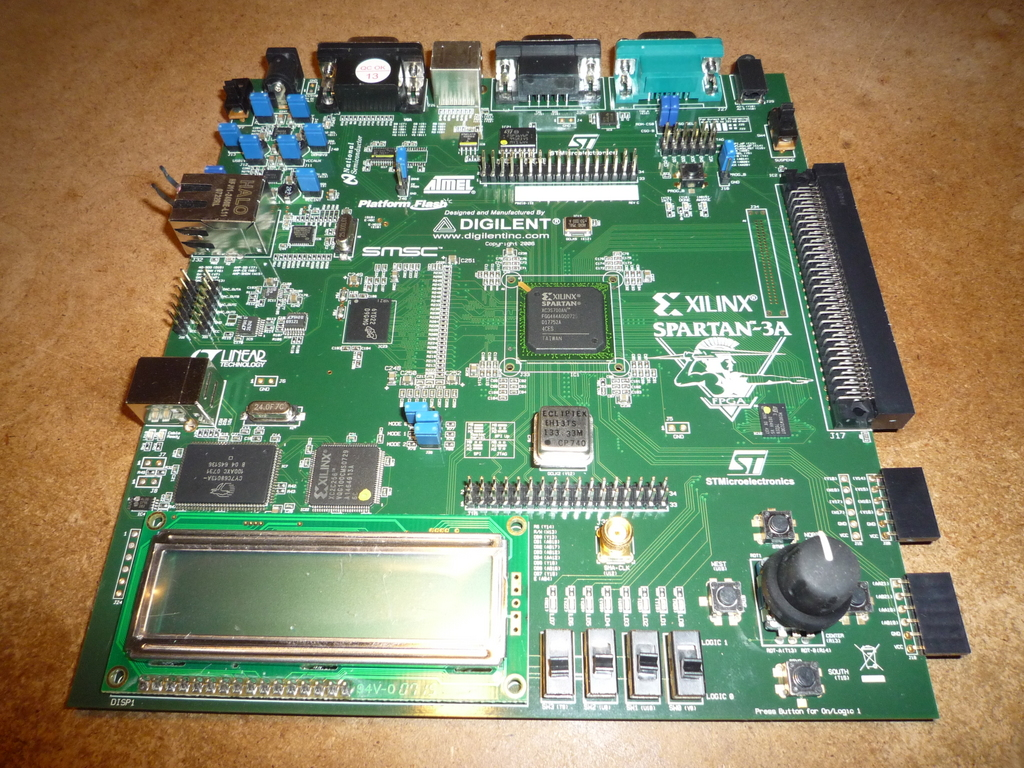
\includegraphics{grafika/spartan3an.jpg}
   \caption{Xilnix Spartan-3AN Starter Kit}
\end{figure}

Celem pracy jest oprogramowanie za pomocą języka opisu sprzętu (Verliog) układów używanych podczas zajęć laboratoryjnych z Projektowanie Systemów Cyfrowych. Praca polegałaby na przygotowaniu zestawu syntezowalnych bloków HDL do wszystkich elementów płytki „Xilnix Spartan-3AN Starter Kit” (www.xilinx.com/products/devkits/HW-SPAR3AN-SK-UNI-G.htm). Dodatkowo należy opracować modele behawioralne służące do testowania poprawności kodu (poszczególnych modułów sprzętu) tworzonego przez studentów podczas zajęć. Podsumowaniem całości ma być projekt kompleksowo demonstrujący możliwości wyżej wspomnianego sprzętu.

Utworzone moduły behawioralne muszą jak najwierniej odzwierciedlać zachowania układów występujących na płytce.
Znajdą wtedy zastosowanie w uruchamianych symulacjach przebiegów czasowych danej konfiguracji układu programowalnego FPGA. Dzięki nim możliwe będzie stwierdzenie czy dla zsyntetyzowanej konfiguracji stany linii FPGA prowadzące do konkretnego układu płytki przebiegają poprawnie i czy zachodzi pożądana komunikacja poprzez generowanie przez te moduły stosownych komunikatów. W ten sposób studenci będą mogli testować poprawność działania utworzonej przez siebie konfiguracji bez fizycznego dostępu do sprzętu.
%zsyntetysowanej/wysyntetyzowanej

\section{Elektronika cyfrowa}
Elektronika cyfrowa operuje na prądach zmiennych, nieokresowych o stałych napięciach. Odróżniane są jedynie dwa stany logiczne - stan wysokiego potencjału będący logicznym wyrażeniem prawdy oraz stan niskiego potencjału - odpowiednik fałszu. Tworzona jest sieć logiczna operująca na zadanych stanach i dostarczająca rezultat działania na swoich wyjściach. Sieć często pracuje w rytm podsuniętego zegara - okresowego sygnału prostokątnego o 50\% wypełnieniu. Sieć może zapamiętać pewne stany wejściowe i brać je pod uwagę w wyliczaniu następnych cykli.

\subsection{Logika cyfrowa}
Każda sieć zbudowana jest jedynie z kilku typów podstawowych operacji logicznych.

\subsubsection{Negacja}
Element negujący zawsze zaprzeczy każdej podanej treści i podmieni jej zawartość na przeciwną.

\begin{table}[h!]
\centering

\begin{minipage}{5.5cm}
\centering

\begin{tabular}{ | c || r | }
  \hline
  $p$ & $\lnot p$ \\ \hline
  0 & 1 \\
  1 & 0 \\
  \hline
\end{tabular}
\end{minipage}
\begin{minipage}{11cm}
\begin{tabular}{  c r }
  & \\
\end{tabular}
\end{minipage}
\end{table}

\subsubsection{Koniunkcja}

Koniunkcja wyznacza prawdę tylko, gdy wszyscy jej doradcy jednogłośnie ją potwierdzają.

\begin{table}[h!]
\centering

\begin{minipage}{5.5cm}
\centering

\begin{tabular}{ | c | c || c | }
  \hline
  $p$ & $q$ & $p \land q$ \\ \hline
  0 & 0 & 0 \\
  0 & 1 & 0 \\
  1 & 0 & 0 \\
  1 & 1 & 1 \\
  \hline
\end{tabular}
\end{minipage}
\begin{minipage}{11cm}
   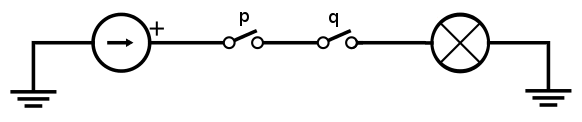
\includegraphics[width=10cm]{grafika/obwody/circuit-and.png}
   \caption*{Demonstracja koniunkcji zrealizowanej na połączeniach}
\end{minipage}
\end{table}

\subsubsection{Alternatywa}
Alternatywa powiela prawdę, jeśli tak stanowi co najmniej jeden jej doradca.

\begin{table}[h!]
\centering

\begin{minipage}{5.5cm}
\centering

\begin{tabular}{ | c | c || c | }
  \hline
  $p$ & $q$ & $p \lor q$ \\ \hline
  0 & 0 & 0 \\
  0 & 1 & 1 \\
  1 & 0 & 1 \\
  1 & 1 & 1 \\
  \hline
\end{tabular}
\end{minipage}
\begin{minipage}{11cm}
   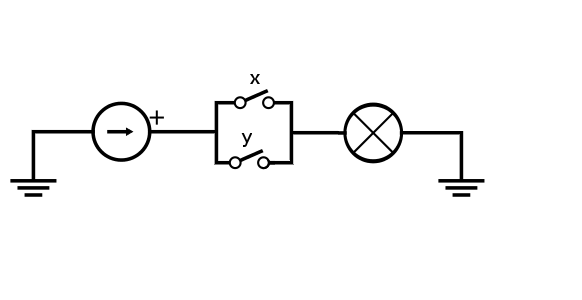
\includegraphics[width=10cm]{grafika/obwody/circuit-or.png}
   \caption*{Demonstracja alternatywy zrealizowanej na połączeniach}
\end{minipage}
\end{table}


\newpage

\subsubsection{Alternatywa wykluczająca}
Alternatywa wykluczająca przechyli się ku prawdzie, gdy jest ona głoszona przez nieparzystą liczbę doradców.

\begin{table}[h!]
\centering

\begin{minipage}{5.5cm}
\centering

\begin{tabular}{ | c | c || c | }
  \hline
  $p$ & $q$ & $p \oplus q$ \\ \hline
  0 & 0 & 0 \\
  0 & 1 & 1 \\
  1 & 0 & 1 \\
  1 & 1 & 0 \\
  \hline
\end{tabular}
\end{minipage}
\begin{minipage}{11cm}
\begin{tabular}{  c r }
  & \\
\end{tabular}
\end{minipage}
\end{table}

\subsubsection{Zasada precedencji}
Pomiędzy zdaniami logicznymi używa się nawiasowania dla zmiany pierwszeństwa ich ewaluacji. Naturalnym biegiem jest rozpatrywanie ich według przyjętej hierarchii $\lnot \land \lor \iff$.

\subsubsection{Prawa De Morgana}
Do formułowania praw należy wprowadzić kolejny symbol logiczny równoważności. W zasadzie jest on zaprzeczeniem poznanej już alternatywy wykluczającej.

\begin{table}[h!]
\centering

\begin{minipage}{5.5cm}
\centering

\begin{tabular}{ | c | c || c | }
  \hline
  $p$ & $q$ & $p \iff q$ \\ \hline
  0 & 0 & 1 \\
  0 & 1 & 0 \\
  1 & 0 & 0 \\
  1 & 1 & 1 \\
  \hline
\end{tabular}
\end{minipage}
\begin{minipage}{11cm}
\begin{tabular}{  c r }
  & \\
\end{tabular}
\end{minipage}
\end{table}

\textbf{I prawo De Morgana} to prawo zaprzeczania koniunkcji. Negacja koniunkcji jest równoważna alternatywie negacji.

$\lnot (p \land q) \iff (\lnot p \lor \lnot q)$

\begin{table}[h!]
\centering

\begin{minipage}{15cm}
\centering

\begin{tabular}{ | c | c || c | c || c | c | c || c | }
  \hline
  $p$ & $q$ & $p \land q$ & $\lnot (p \land q)$ & $\lnot p$ & $\lnot q$ & $(\lnot p \lor \lnot q)$ & $\lnot (p \land q) \iff (\lnot p \lor \lnot q)$ \\ \hline
  0 & 0 & 0 & 1 & 1 & 1 & 1 & 1 \\
  0 & 1 & 0 & 1 & 1 & 0 & 1 & 1 \\
  1 & 0 & 0 & 1 & 0 & 1 & 1 & 1 \\
  1 & 1 & 1 & 0 & 0 & 0 & 0 & 1 \\
  \hline
\end{tabular}

\end{minipage}
\begin{minipage}{0.5cm}
\begin{tabular}{  c r }
  & \\
\end{tabular}
\end{minipage}
\end{table}


\textbf{II prawo De Morgana} to prawo zaprzeczenia alternatywy. Negacja alternatywy jest równoważna koniunkcji negacji


$\lnot (p \lor q) \iff (\lnot p \land \lnot q)$

\begin{table}[h!]
\centering

\begin{minipage}{15cm}
\centering

\begin{tabular}{ | c | c || c | c || c | c | c || c | }
  \hline
  $p$ & $q$ & $p \lor q$ & $\lnot (p \lor q)$ & $\lnot p$ & $\lnot q$ & $(\lnot p \land \lnot q)$ & $\lnot (p \lor q) \iff (\lnot p \land \lnot q)$ \\ \hline
  0 & 0 & 0 & 1 & 1 & 1 & 1 & 1 \\
  0 & 1 & 1 & 0 & 1 & 0 & 0 & 1 \\
  1 & 0 & 1 & 0 & 0 & 1 & 0 & 1 \\
  1 & 1 & 1 & 0 & 0 & 0 & 0 & 1 \\
  \hline
\end{tabular}

\end{minipage}
\begin{minipage}{0.5cm}
\begin{tabular}{  c r }
  & \\
\end{tabular}
\end{minipage}
\end{table}


Prawa te są bardzo pomocne do optymalizacji sieci.


\subsection{Bramki logiczne}
Są to układy scalone realizujące wyspecyfikowane przez producenta operacje logiczne. Na samych połączeniach przewodów można jedynie osiągnąć logikę koniunkcji lub alternatywy. Nie da się jednak obecnemu w sieci sygnałowi zaprzeczyć. Można by problem obejść używając mechanicznych przekaźników. Właściwsze mogą okazać się tranzystory, tudzież ich zestawy odpowiednio połączone i zatopione w gotowych scalakach nazywanych bramkami logicznymi.

\begin{table}[h!]
\centering
\begin{minipage}{2.5cm}
   \centering
   
\includegraphics{grafika/obwody/not.png}
   \caption*{negacja}
\end{minipage}
\begin{minipage}{2.5cm}
   \centering
   
\includegraphics{grafika/obwody/and.png}
   \caption*{koniunkcja}
\end{minipage}
\begin{minipage}{2.5cm}
   \centering
   
\includegraphics{grafika/obwody/or.png}
   \caption*{alternatywa}
\end{minipage}
\begin{minipage}{2.5cm}
   \centering
   
\includegraphics{grafika/obwody/xor.png}
   \caption*{alternatywa wykluczająca}
\end{minipage}
\begin{minipage}{2.5cm}
   \centering
   
\includegraphics{grafika/obwody/nand.png}
   \caption*{zaprzeczona koniunkcja}
\end{minipage}
\begin{minipage}{2.5cm}
   \centering
   
\includegraphics{grafika/obwody/nor.png}
   \caption*{zaprzeczona alternatywa}
\end{minipage}

\caption*{Oznaczenia schematyczne operacji logicznych}
\end{table}

Dokumentacja układu określa położenia pinów wejściowych i wyjściowych każdej z dostępnych operacji.

\begin{table}[h!]
\centering
\begin{minipage}{5cm}
   \centering
   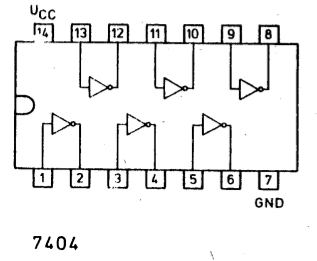
\includegraphics[width=5cm]{grafika/cemi/6not.png}
   %% \caption*{negacja}
\end{minipage}
\begin{minipage}{5cm}
   \centering
   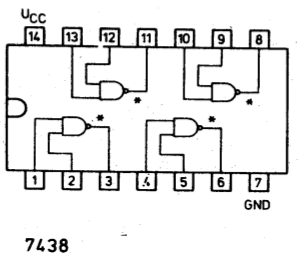
\includegraphics[width=5cm]{grafika/cemi/4nand.png}
   %% \caption*{negacja}
\end{minipage}
\begin{minipage}{5cm}
   \centering
   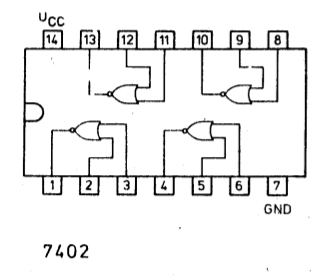
\includegraphics[width=5cm]{grafika/cemi/4nor.png}
   %% \caption*{negacja}
\end{minipage}

\begin{minipage}{5cm}
   \centering
   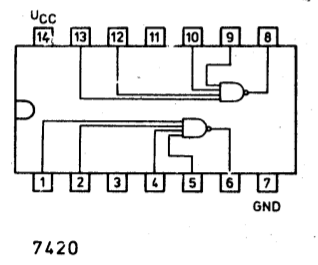
\includegraphics[width=5cm]{grafika/cemi/2nand.png}
   %% \caption*{negacja}
\end{minipage}
\begin{minipage}{5cm}
   \centering
   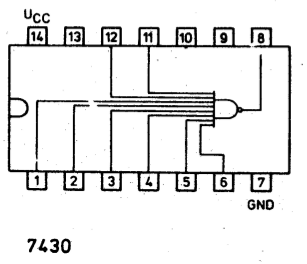
\includegraphics[width=5cm]{grafika/cemi/1nand.png}
   %% \caption*{negacja}
\end{minipage}
\begin{minipage}{5cm}
   \centering
   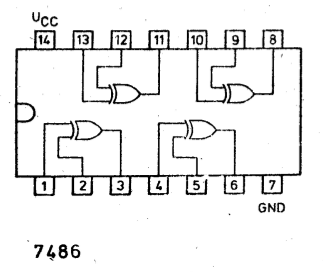
\includegraphics[width=5cm]{grafika/cemi/4xor.png}
   %% \caption*{negacja}
\end{minipage}

\caption*{Przykładowe bramki logiczne polskiej PRL-owskiej produkcji firmy CEMI}
\end{table}

\begin{figure}[htb]
   \centering
   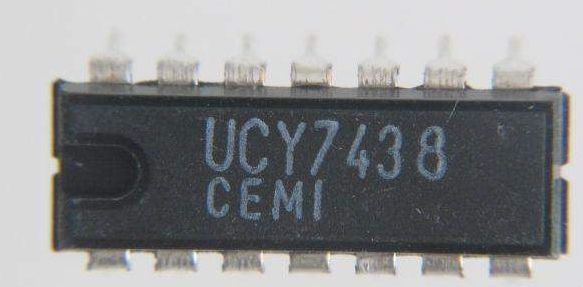
\includegraphics[width=4cm]{grafika/cemi/ucy7438.jpg}
   \caption*{Egzemplarz bramki logicznej}
\end{figure}

\subsubsection{Hazard}
Zadanie nowego stanu wejścia wymaga czasu na przełączenie się wewnętrznych tranzystorów zanim ustali się właściwy wynik na wyjściu. Opóźnienie to nazywane jest czasem propagacji bramki. W tych krótkich momentach stany wyjść są nieustalone.



\subsection{Systemy liczbowe}

Cyfry są zestawem symboli danego systemu liczbowego ułożonych w określonym porządku według rosnących znaczeń. Przyjęło się uważać za naturalny system o dziesięciu cyfrach.

$0_{min}$ $1$ $2$ $3$ $4$ $5$ $6$ $7$ $8$ $9^{max}$

Końce porządku wyznaczają symbole najmniejszy i największy.

Liczba jest nieskończonym ciągiem cyfr.

Algorytm nieskończonej inkrementacji liczby zaczyna od jej postaci najmniejszej.

$0_{min}$ ... $0_{min}$ $0_{min}$ $0_{min}$

Przegląda ciąg zaczynając od najbardziej skrajnego prawego miejsca poszukując pierwszego symbolu niemaksymalnego. Natrafia na niego natychmiast.

Element ten jest sukcesywnie podmieniany na symbol starszy stopniem w szeregu.

$0_{min}$ ... $0_{min}$ $0_{min}$ $1$

$0_{min}$ ... $0_{min}$ $0_{min}$ $2$

$0_{min}$ ... $0_{min}$ $0_{min}$ $3$

$0_{min}$ ... $0_{min}$ $0_{min}$ $4$

$0_{min}$ ... $0_{min}$ $0_{min}$ $5$

$0_{min}$ ... $0_{min}$ $0_{min}$ $6$

$0_{min}$ ... $0_{min}$ $0_{min}$ $7$

$0_{min}$ ... $0_{min}$ $0_{min}$ $8$

$0_{min}$ ... $0_{min}$ $0_{min}$ $9^{max}$

Po wyczerpaniu puli na pierwszej pozycji, zajrzy na następną z kolei i tam napotka symbol niemaksymalny do podmiany na większy. Wszystkie symbole na prawo od znalezionej pozycji muszą zostać zminimalizowane.

$0_{min}$ ... $0_{min}$ $1$ $0_{min}$

Ponownie można podmieniać symbole na pierwszej pozycji zgodnie z porządkiem aż do osiągnięcia symbolu maksymalnego. Wtedy ponownie poszukiwana będzie pozycja pierwsza niemaksymalna i tu algorytm się zapętla.

$0_{min}$ ... $0_{min}$ $1$ $1$

\subsubsection{Liczby binarne}

Stosując tą samą zasadę postępowania można odliczać liczby w dowolnym systemie o uznanym porządku symboli. Logika binarna skraca pulę symboli do dwóch możliwości, odróżniając jedynie sybmole najmniejszy i największy.

$0_{min}$ $1^{max}$

Odliczanie zawsze startuje od nieskończonego ciągu symboli najmniejszych.

$0_{min}$ ... $0_{min}$ $0_{min}$ $0_{min}$

Już po pierwszej iteracji pula zostaje wyczerpana.

$0_{min}$ ... $0_{min}$ $0_{min}$ $1^{max}$

Należy użyć kolejnej, drugiej pozycji i wyzerować poprzednie.

$0_{min}$ ... $0_{min}$ $1^{max}$ $0_{min}$

Iteracja pierwszej pozycji

$0_{min}$ ... $0_{min}$ $1^{max}$ $1^{max}$

I znowu przepełnienie, tym razem już dwóch pierwszych pozycji. Należy poruszyć trzecią jako pierwszą niemaksymalną.

$0_{min}$ ... $1^{max}$ $0_{min}$ $0_{min}$

Na dwóch pierwszych pozycjach zostają powtórzone trzy poprzednie kroki, po czym należy sięgnąć na pozycję czwartą i powtórzyć kroki jej dotychczasowe. I tak do nieskończoności.


\begin{table}[h!]
\centering
\begin{tabular}{ | c | c | c | c |}
  \hline
  dwójkowy & ósemkowy & dziesiętny & szesnastkowy \\ \hline
  00000 & 00 & 00 & 00 \\
  00001 & 01 & 01 & 01 \\
  00010 & 02 & 02 & 02 \\
  00011 & 03 & 03 & 03 \\
  00100 & 04 & 04 & 04 \\
  00101 & 05 & 05 & 05 \\
  00110 & 06 & 06 & 06 \\
  00111 & 07 & 07 & 07 \\
  01000 & 10 & 08 & 08 \\
  01001 & 11 & 09 & 09 \\
  01010 & 12 & 10 & 0A \\
  01011 & 13 & 11 & 0B \\
  01100 & 14 & 12 & 0C \\
  01101 & 15 & 13 & 0D \\
  01110 & 16 & 14 & 0E \\
  01111 & 17 & 15 & 0F \\
  10000 & 20 & 16 & 10 \\
  10001 & 21 & 17 & 11 \\
  10010 & 22 & 18 & 12 \\
  10011 & 23 & 19 & 13 \\
  10100 & 24 & 20 & 14 \\
  \hline
\end{tabular}
\caption*{Tabela odzwierciedla odliczanie w paru systemach liczbowych}
\end{table}


\subsection{Układy kombinacyjne}

Są to układy cyfrowe, które nie zapamiętują stanów pośrednich obliczeń wewnątrz sieci. Stany wyjść są zależne jedynie od stanów bieżących wejść. Są ich funkcją logiczną.

Linie wejść/wyjść układów cyfrowych często są liczbami reprezentowanymi w systemie dwójkowym. Uprzednio zaprezentowane nieskończone ciągi cyfr są modelem matematycznym nie mającym odzwierciedlenia w realnych układach elektronicznych na współczesnym etapie rozwoju techniki. Maszyny przejawiają skończoną precyzję obliczeń wykonywaną w skończonym czasie.

W systemie dwójkowym (binarnym) pojedynczą cyfrę nazywa się jednym bitem informacji. Na jednym bicie można zapisać jedną z dwóch możliwych wartości $0_{min}$ lub $1^{max}$. Na dwóch bitach zapisuje się wszystkie dwie możliwości pierwszego bitu zdwukrotnione dwiema możliwościami bitu drugiej pozycji. Razem 4 możliwości. Dodając trzeci bit, również ilość możliwości się dubluje dając 8. I tu uwidacznia się pewna reguła - na $n$ bitach można zapisać jedną z $2^n$ możliwych liczb. Odliczając od zera, liczbą największą będzie $2^n-1$.

\subsubsection{Jedno-bitowy układ dodający}

Układ ten dodaje dwa jedno-bitowe sygnały nazwane $A$ i $B$. Jeśli oba wejścia wystawią stan wysoki, wtedy wynik $2$ w systemie binarnym $(10)_2$ jest liczbą dwucyfrową wymagającą dwóch wyjściowych linii $S$ i starszej $C$ (informującej też o przepełnieniu).

Po sformułowaniu tablicy prawdy łatwo zauważyć, że linia $S$ jest alternatywą wykluczającą wejść, natomiast $C$ jest ich koniunkcją.

\begin{table}[h!]
\centering

\begin{minipage}{5.5cm}
\centering

\begin{tabular}{ | c | c || c | c | }
  \hline
  $A$ & $B$ & $S$ & $C$ \\ \hline
  0 & 0 & 0 & 0 \\
  0 & 1 & 1 & 0 \\
  1 & 0 & 1 & 0 \\
  1 & 1 & 0 & 1 \\
  \hline
\end{tabular}
\end{minipage}
\begin{minipage}{11cm}
   \centering
   \includesvg[svgpath = grafika/obwody/]{Half_Adder}
   \caption*{Sieć logiczna jedno-bitowego układu dodającego}
\end{minipage}
\end{table}


\subsubsection{Wielobitowy układ dodający}

Dodawanie liczb złożonych z większej liczby bitów wymaga właściwego obchodzenia się z bitem przepełnienia. Mechanizm ujawnia dodawanie pisemne, które jest analogiczne jak w systemie dziesiętnym. Dla przykładu użyte zastaną liczby $A = 14 = (1110)_2$ oraz $B = 7 = (0111)_2$. Indeks przy oznaczeniu liczby odnosi się do cyfry na wskazanej pozycji bitu.

\begin{table}[h!]
\centering

\begin{minipage}{5.5cm}
\centering

\begin{tabular}{  c  c  c  c  c  c  }
      & 1 & 1 & 1 &   &   \\
      &   & 1 & 1 & 1 & 0 \\
  $+$ &   & 0 & 1 & 1 & 1 \\
  \hline
      & 1 & 0 & 1 & 0 & 1 \\
\end{tabular}
\end{minipage}
\begin{minipage}{11cm}
\begin{tabular}{  c  c  c  c  c  c  }
      & $C_4$ & $C_3$ & $C_2$ & $C_1$ &       \\
      &       & $A_3$ & $A_2$ & $A_1$ & $A_0$ \\
  $+$ &       & $B_3$ & $B_2$ & $B_1$ & $B_0$ \\
  \hline
      &       & $S_3$ & $S_2$ & $S_1$ & $S_0$ \\
\end{tabular}
\end{minipage}
\end{table}

Najpierw dodawane są najmłodsze bity $A_0 = 0$ i $B_0 = 1$, a ich wynikiem, zgodnie z tabelą dodawania jedno-bitowego, jest $S_0 = 1$. W następnej kolumnie występują dwa stany wysokie, co zgodnie z tabelą wynosi $0$ dla $S_1$, ale ustawiany jest bit przepełnienia $C_2$. Dla trzeciej kolumny ponownie oba wejścia są wysokie, jednak należy także wziąść pod uwagę przepełnienie $C_2$ z poprzedniego kroku. Ta sytuacja dotąd nie została uwzględniona. Należy dla niej zaprezentować ogólniejszą tabelę prawdy uwzględniającą bit przepełnienia z poprzedniego dodawania.

\begin{table}[h!]
\centering

\begin{minipage}{5.5cm}
\centering

\begin{tabular}{ | c | c | c || c | c | }
  \hline
  $A$ & $B$ & $C_{in}$ & $S$ & $C_{out}$ \\ \hline
  0 & 0 & 0 & 0 & 0 \\
  0 & 1 & 0 & 1 & 0 \\
  1 & 0 & 0 & 1 & 0 \\
  1 & 1 & 0 & 0 & 1 \\
  0 & 0 & 1 & 1 & 0 \\
  0 & 1 & 1 & 0 & 1 \\
  1 & 0 & 1 & 0 & 1 \\
  1 & 1 & 1 & 1 & 1 \\
  \hline
\end{tabular}
\end{minipage}
\begin{minipage}{11cm}
   \centering
   \includesvg[svgpath = grafika/obwody/]{Full-adder_logic_diagram_old}
   \caption*{Sieć logiczna pojedynczego ogniwa wielobitowego układu dodającego.}
\end{minipage}
\end{table}

Teraz widać, że ogólna postać dodawania ma trzy wejścia - dwa są bitami z obu składników na odpowiadających sobie pozycjach, trzeci sygnał jest wartością przepełnienia z dodawania na poprzedniej pozycji.

Tak więc w kolumnie trzeciej wystąpiła sytuacja, gdzie oba wejścia są wysokie jak również i bit przepełnienia. Według nowej tablicy trzy jedynki na wejściu dają dwie na wyjściu.

Czwarta kolumna otrzymuje przepełnienie i jedną jedynkę, co oznacza zero dla $S_3$ oraz ostatnie przepełnienie $C_4$. Wynikiem jest $21 = (10101)_2$, co wymaga zapisu na 5 bitach. Ostatni bit przepełnienia zapewnia brakujący piąty bit wyniku, dzięki czemu suma jest właściwa w postaci $C_4 S_3 S_2 S_1 S_0$.

\begin{figure}[htb]
   \centering
   \includesvg[width=15cm,svgpath = grafika/obwody/]{4-bit_ripple_carry_adder}
   \caption*{4-bitowy układ dodający zbudowany jest z 4 ogniw}
\end{figure}


\subsubsection{Multiplexer}


\subsubsection{Jedno-bitowy układ porównujący}

Układ porównujący stwierdza, czy dwa wejściowe sygnały $A$ i $B$ są sobie równe linią $=$. A jeśli nie są, wtedy określi który z nich reprezentuje większą wartość za pomocą wyprowadzeń $<$ oraz $>$.


\begin{table}[h!]
\centering

\begin{minipage}{6.5cm}
\centering

\begin{tabular}{ | c | c || c | c | c | }
  \hline
  $A$ & $B$ & $A<B$ & $A=B$ & $A>B$ \\ \hline
  0 & 0 & 0 & 1 & 0 \\
  0 & 1 & 1 & 0 & 0 \\
  1 & 0 & 0 & 0 & 1 \\
  1 & 1 & 0 & 1 & 0 \\
  \hline
\end{tabular}
\end{minipage}
\begin{minipage}{10cm}
   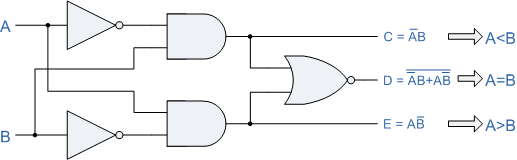
\includegraphics[width=8.5cm]{grafika/obwody/cmp.png}
   \caption*{Sieć logiczna jedno-bitowego układu porównującego}
\end{minipage}
\end{table}


\subsubsection{Wielobitowy układ porównujący}

Równość dwóch dowolnych wartości $n$-bitowych stwierdza się, jeśli wszystkie odpowiadające sobie bity są sobie równe.

$x_i= A_i \cdot B_i + \overline{A}_i \cdot \overline{B}_i.$

$(A=B) = x_nx_{n-1} (...) x_2x_1x_0$

Nierówność stwierdza się porównując odpowiadające sobie bity kolejno poczynając od najstarszego aż do wykrycia pierwszej nieprawidłowości. Znak $<$ lub $>$ nierówności klaruje się według porównania jedno-bitowego na znalezionej pozycji.

$(A>B)=A_3 \cdot \overline{B}_3+x_3 A_2 \overline{B}_2+x_3 x_2 A_1 \overline{B}_1+x_3x_2x_1 A_0 \overline{B}_0$

$(A<B)=\overline{A}_3 \cdot B_3+x_3 \overline{A}_2 B_2+x_3 x_2 \overline{A}_1 B_1+x_3x_2x_1 \overline{A}_0 B_0$


\begin{table}[h!]
\centering

\begin{minipage}{9cm}
\centering

\begin{tabular}{ | c | c | c | c || c | c | c | }
  \hline
  $A_1$ & $A_0$ & $B_1$ & $B_0$ & $A<B$ & $A=B$ & $A>B$ \\ \hline
  0 & 0 & 0 & 0 & 0 & 1 & 0 \\
  0 & 0 & 0 & 1 & 1 & 0 & 0 \\
  0 & 0 & 1 & 0 & 1 & 0 & 1 \\
  0 & 0 & 1 & 1 & 1 & 0 & 0 \\ \hline
  0 & 1 & 0 & 0 & 0 & 0 & 1 \\
  0 & 1 & 0 & 1 & 0 & 1 & 0 \\
  0 & 1 & 1 & 0 & 0 & 0 & 1 \\
  0 & 1 & 1 & 1 & 1 & 0 & 0 \\ \hline
  1 & 0 & 0 & 0 & 0 & 0 & 1 \\
  1 & 0 & 0 & 1 & 0 & 0 & 1 \\
  1 & 0 & 1 & 0 & 0 & 1 & 0 \\
  1 & 0 & 1 & 1 & 1 & 0 & 0 \\ \hline
  1 & 1 & 0 & 0 & 0 & 0 & 1 \\
  1 & 1 & 0 & 1 & 0 & 0 & 1 \\
  1 & 1 & 1 & 0 & 0 & 0 & 1 \\
  1 & 1 & 1 & 1 & 0 & 1 & 0 \\
  \hline
\end{tabular}
\end{minipage}
\begin{minipage}{7.5cm}
   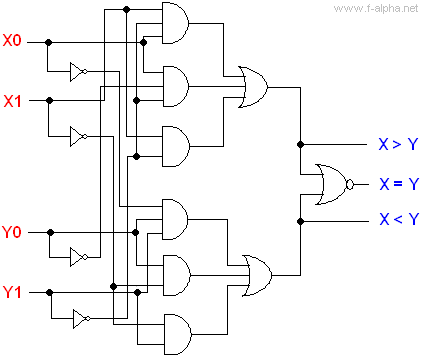
\includegraphics[width=7cm]{grafika/obwody/circuit_diagram_2_bit_magnitude_comparator.png}
   \caption*{Sieć logiczna dwu-bitowego układu porównującego}
\end{minipage}
\end{table}



\subsection{Układy sekwencyjne}

W układach sekwencyjnych do pewnych sygnałów wejściowych są przyłączone niektóre wyjścia sprzężeniem zwrotnym. Dzięki temu na bieżący wynik obliczeń wpływają obliczenia uprzednie. Zachodzi efekt pamięci - sieć pamięta swoje poprzednie stany.

\subsubsection{Zatrzask SR}

\begin{table}[h!]
\centering

\begin{minipage}{6.5cm}
\centering

\begin{tabular}{ | c | c || c | c | }
  \hline
  $\lnot S$ & $\lnot R$ & $Q$ & $\lnot Q$ \\ \hline
  0 & 0 & x & x \\
  0 & 1 & 1 & 0 \\
  1 & 0 & 0 & 1 \\
  1 & 1 & $Q_{n-1}$ & $\lnot Q_{n-1}$ \\
  \hline
\end{tabular}
\end{minipage}
\begin{minipage}{10cm}
   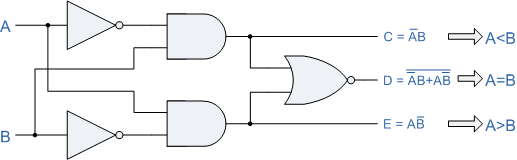
\includegraphics[width=8.5cm]{grafika/obwody/cmp.png}
   \caption*{Sieć logiczna jedno-bitowego układu porównującego}
\end{minipage}
\end{table}

Przerzutnik SR zbudowany jest z dwóch bramek NOR lub NAND. Wynik wyjścia jednej bramki skierowany jest ponownie do wejścia drugiej. Dzięki temu pozostawiając układ w stanie neutralnym, stale utrzymuje on na swoim wyjściu ostatnio wybrany stan. Stan wybiera się wytrącając układ ze stanu neutralnego krótkim zwarciem linii $S$ lub $R$ do masy. Jeśli obie linie naraz zostaną zwarte, wtedy stan wyjściowy uzależniony jest od wewnętrznych hazardów i przyjmuje się go za nieustalony.

\subsubsection{Przerzutnik D}

\begin{table}[h!]
\centering

\begin{minipage}{6.5cm}
\centering

\begin{tabular}{ | c | c || c | }
  \hline
  $D$ & $C$ & $Q$ \\ \hline
  x & 0 & $Q_{n-1}$ \\
  0 & 1 & 0 \\
  1 & 1 & 1 \\
  \hline
\end{tabular}
\end{minipage}
\begin{minipage}{10cm}
   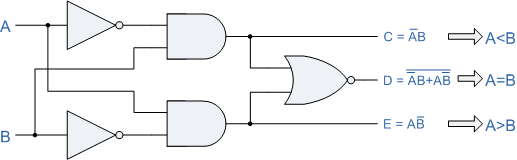
\includegraphics[width=8.5cm]{grafika/obwody/cmp.png}
   \caption*{Sieć logiczna jedno-bitowego układu porównującego}
\end{minipage}
\end{table}

Przerzutnik D jest rozszerzeniem zatrzasku SR o 2 dodatkowe bramki uniemożliwiające osiągnięcie stanu zabronionego obarczonego nieprzewidywalnymi hazardami. Oczekuje on przyłączenia linii danych $D$ oraz zegarowej $C$. W chwilach wysokiego stanu zegara, stale przepisuje on daną $D$ na wyjście. Gdy stan zegara stanie się niski, wtedy ostatnia przepisana i 'zapamiętana' wartość $D$ jest utrzymywana na wyjściu.


Dwa przerzutniki D czułe na przeciwne poziomy zegara łączy się kaskadowo. Efektem jest przerzutnik czuły na zbocze zegara. Kierunek zbocza wyznacza kolejność podłączenia przerzutników.

\subsubsection{Rejestr}

Rejestr jest układem pamięciowym przechowującym bity informacji. Jego budowę można oprzeć na zestawie przerzutników typu D łącząc je równolegle.

\subsubsection{Licznik}

Licznik to układ inkrementujący liczbę przedstawianą binarnie na wyjściu w takt dostarczanego zegara. Zbudować go można łącząc szeregowo przerzutniki typu D. Do pierwszego dostarcza się sygnał zegarowy, a sygnałem $C$ dla kolejnych jest wyjście $Q$ z poprzedniego. Każdemu przerzutnikowi z osobna zwiera się wyjście $\lnot Q$ z wejściem $D$. Inkrementowana liczba ujawnia się w ciągu $Q_{n-1} Q_{n-2} .. Q_{0}$.

\subsection{FPGA}

Field Programmable Gate Array jest układem elektronicznym pozwalającym na skonfigurowanie jego zachowania. Konfiguracja taka jest zestawem wygenerowanych danych dostarczonych do FPGA i określa logikę, według której układ ma pracować. Ekwiwalentną logikę przedstawić można układem bramek logicznych i przerzutników.

\subsubsection{Architektura}

W układzie FPGA wyszczególnić można elementy nazywane blokami logicznymi, które zwarte są ze sobą siecią konfigurowalnych połączeń. Linie wejściowe bloku logicznego poprowadzone poprzez multipleksery do przerzutników* stają się indeksem komórki pamięci. Wartość tam zapisana będzie wynikiem działania sieci. Pamięć ta przechowuje możliwe stany wyjściowe dla wszystkich kombinacji wejść, stąd nazywana jest tablicą przeszukiwań LUT. Tym sposobem odwzorować można dowolną logikę kombinacyjną.

Układy FPGA pozwalają na więcej, także odzwierciedlają logikę sekwencyjną. Wynik z tablicy LUT jest poprowadzony przez multiplekser. Jego konfiguracja powoduje bezpośrednie wyprowadzenie sygnału z bloku logicznego lub przeprowadzenie go przez dedykowany przerzutnik (taktowany wspólnym zegarem dla wszystkich bloków). W tym przypadku bloki logiczne spełniają także funkcję pamięciową.

Logika programowalna przechowuje konfigurację swojego działania w rozproszonych w układzie pamięciach RAM. Zapis pamięci o połączeniach między blokami logicznymi, zawartością ich tablic LUT oraz konfiguracją ich multiplekserów dla przerzutników jest konfiguracją układu FPGA. Od zadanej konfiguracji zależy działanie całego układu elektronicznego.

\subsection{Języki Opisu Sprzętu}

Modelowanie pojedynczych bitów w poszczególnych pamięciach RAM układu FPGA byłoby niezwykle żmudnym i błędogennym zadaniem, a powstały efekt końcowy byłby nieprzenośny na układy nowsze lub innych producentów. Stąd narosła potrzeba narzędzia do wygenerowania konfiguracji FPGA dla wskazanego chipsetu bazując na dostarczonym modelu pożądanego funkcjonowania sprzętu. Model taki sporządzany jest w języku opisu sprzętu elektronicznego. Najpopularniejsze to VHDL i Verilog oraz wzbogacony o rozszerzenia obiektowe SystemVerilog.

Języki te ze swojej natury modelują procesy współbieżne synchronizowane na zboczach zegara taktującego cały układ.

\subsubsection{Verilog}

Verilog dysponuje dwoma podstawowymi typami danych. Pierwszym jest rejestr, oto jego deklaracja
\begin{lstlisting}[label=reg,caption=Rejestr]
reg rejestr_jednobitowy;
reg rejestr_jednobitowy_z_przypisana_wartoscia = 1'b1;
reg [7:0] rejestr_8bitowy = 8'haa;
reg [7:0] pamiec_256_elementow_1bajtowych [255:0];
\end{lstlisting}
Rejestry dane przechowują. Można je wpisywać i odczytywać. Prawa strona przypisania zawiera liczbę bitów przedstawianej liczby, po apostrofie definiuje jej system liczbowy zapisu (z dostępnych binarnego $b$, heksadecymalnego $h$ i dziesiętnego $d$), na końcu przedstawia samą liczbę.

Drugim typem danych jest połączenie tworzące więź z rejestrem macierzystym.
\begin{lstlisting}[label=reg,caption=Polaczenie]
wire polaczenie_jednobitowe = rejestr_jednobitowy;
wire [2:0] ekstrakcja_3bitow_z_rejestru = rejestr_8bitowy[3:1];
wire [7:0] konkatenacja_rejestrow = {rejestr_8bitowy[6:0], rejestr_jednobitowy};
wire kombinatoryka = (rejestr_jednobitowy) ? rejestr_8bitowy[4] : 1'b1;
\end{lstlisting}
Połączenia mogą jedynie wskazywać dane zamieszczone w rejestrach. Nie można do nich danych zapisywać, do tego celu potrzebny jest bezpośredni dostęp do wskazywanego rejestru. Połączenia mogą ukazywać jedynie interesującą część rejestru dzięki operatorowi ekstrakcji $[ ]$. Mogą też wskazywać części danych zapisanych w kilku innych rejestrach poprzez ich konkatenację $\{\}$. Operator trójargumentowy $? :$ umożliwia zapisanie wyrażeń kombinacyjnych warunkowych.

Dostępne są podstawowe bramki logiczne i poprzez połączenie między nimi modeluje się logikę kombinacyjną, na przykład sumatora jedno bitowego.
\begin{lstlisting}[label=Sum1,caption=Sum1.v]
wire A, B, Cin, Y, Cou;
wire g1_o, g2_o, g3_o, g4_o;

and g1(g1_o, A, B);
xor g4(g4_o, A, B);
and g2(g2_o, Cin, g4_o);
or  g3(Cout, g1_o, g2_o);
xor g5(Y, Cin, g4_0);
\end{lstlisting}

Jednakże właściwsze jest modelowanie na wyższym poziomie abstrakcji zwanym zachowawczym. Syntezator zdolny jest sam podstawić bramki pod logikę, którą się mu przedstawi opisowo.

\begin{lstlisting}[label=Sum1,caption=Sum1.v]
wire A, B, Cin, Y, Cout;

{ Cout, Y } = A + B + Cin;
\end{lstlisting}

Do zamodelowania logiki sekwencyjnej posłużyć się należy rejestrem i blokiem $always$ czułym na zbocze zegara. Zapisywanie wartości do konkretnego rejestru dozwolone jest tylko w jednym, dedykowanym bloku $always$. Przykładowy timer zlicza takty zegara głównego i w równych odstępach czasu informuje o swoich przepełnieniach.
\begin{lstlisting}[label=Timer,caption=Timer.v]
reg [2:0] counter = 3'd0;
wire full = reg == 3'b111;

always @(posedge clk)
   reg <= reg + 1;
\end{lstlisting}

Zadeklarowany został 3-bitowy rejestr $counter$ o początkowej zerowej wartości. Wyjście $full$ sformułowane jest kombinacyjnie i osiąga stan wysoki tylko, gdy licznik jest pełny. Na narastających zboczach dostarczonego z zewnątrz zegara $clk$ wykonuje się blok $always$ inkrementując licznik. W rezultacie sygnał $full$ generowany jest co 8 takt zegara.

Odpowiednikiem obudów układów elektronicznych z wyprowadzonymi pinami są w Verilogu moduły. W ich opisie wyspecyfikowana jest lista wejść i wyjść, a wewnątrz deklarowanego modułu powoływać można instancje innych i modelować połączenia między nimi. Struktura jest hierarchiczna. Zewnętrzne połączenia modułu najwyższego poziomu są wyprowadzeniami pinów FPGA.
\begin{lstlisting}[label=Top,caption=Top.v]
module Top
(
   input wire clk,
   input wire rst,
   input wire [3:0] buttons,
   output wire [7:0] leds
);

wire blink_led;
wire light_all_leds;

Controller controller_(
    .buttons(buttons)
    .blink_led(blink_led),
    .light_all_leds(light_all_leds)
);

Leds leds_(
    .leds(leds),
    .blink_led(blink_led),
    .light_all_leds(light_all_leds)
);

endmodule
\end{lstlisting}

\subsubsection{Procesor}

Na FPGA można zaimplementować logikę arytmetyczną operującą na tych samych rejestrach. Operacje następowałyby pojedynczo w kolejności uzależnionej od ciągu dostarczonych instrukcji nazywanych programem. Co więcej, specjalne instrukcje skoku warunkowego sprawdzałyby stan bieżących obliczeń i od ich zależności mogłyby zakłócić porządek wykonywanego programu zmieniając aktualną pozycję w wykonywanym ciągu instrukcji. Taką konstrukcję nazywa się procesorem.

Przykładowy prosty procesor operuje na jednym 8-bitowym rejestrze zwanym akumulatorem. Ma on dostęp do pamięci RAM również o 8-bitowej szerokości szyny danych. Wszystkie instrukcje są jednakowej długości 2 bajtów i ulokowane są w oddzielnej pamięci PROM. Doprecyzowując procesor ten jest 8-bitowym przedstawicielem rodziny RISC (Reduced Instruction Set Computing) o architekturze harwardzkiej.

Jego możliwości przedstawia tabela

\begin{figure}[htb]
  \centering
\begin{tabular}{ | l | l | p{10cm} | }
  \hline
  Kod maszynowy  & Mnemonik & Opis \\ \hline
  0000 0000 \{OP1\}$_8$  & LDI \{OP1\}$_8$     & Ładuje do akumulatora wartość \{OP1\}$_8$ podaną w instr \\ \hline
  0001 \{ADDR\}$_{12}$   & LD \{ADDR\}$_{12}$ & Ładuje do akumulatora wartość dostępną pod adresem \{ADDR\}$_{12}$ \\ \hline
  0010 \{\{ADDR\}\}$_{12}$   & ST \{\{ADDR\}\}$_{12}$ & Zapisuje wartość z akumulatora pod adresem \{ADDR\}$_{12}$ \\ \hline
  0011 0000 \{OP1\}$_8$  & ADD \{OP1\}$_8$  & Dodaje do akumulatora wartość podaną w instrukcji \{OP1\}$_8$ \\ \hline
  0100 0000 \{OP1\}$_8$  & SUB \{OP1\}$_8$  & Odejmuje od akumulatora wartość podaną w instrukcji \{OP1\}$_8$ \\ \hline
  0101 0000 \{OP1\}$_8$  & AND \{OP1\}$_8$  & Wykonuje na akumulatorze funkcję logiczną AND z operandem \{OP1\}$_8$ \\ \hline
  0110 0000 \{OP1\}$_8$  & OR  \{OP1\}$_8$  & Wykonuje na akumulatorze funkcję logiczną OR  z operandem \{OP1\}$_8$ \\ \hline
  0111 0000 \{OP1\}$_8$  & XOR \{OP1\}$_8$  & Wykonuje na akumulatorze funkcję logiczną XOR z operandem \{OP1\}$_8$ \\ \hline
  1000 0000 00000000 & NOT          & Wykonuje na akumulatorze funkcję logiczną NOT \\ \hline
  1001 0000 00000000 & LR           & Przesuwa wartość akumulatora w lewo \\ \hline
  1010 0000 00000000 & RR           & Przesuwa wartość akumulatora w prawo \\ \hline
  1011 \{ADDR\}$_{12}$ & JMP  \{ADDR\}$_{12}$ & Następne instrukcje procesor wykonana spod adresu \{ADDR\}$_{12}$ \\ \hline
  1100 \{ADDR\}$_{12}$ & JMPZ \{ADDR\}$_{12}$ & Jeśli w akumulatorze jest wartość zero, to następne instrukcje procesor wykonana spod adresu \{ADDR\}$_{12}$ \\ \hline
\end{tabular}
\end{figure}

Są instrukcje bezargumentowe jak zaprzeczenie NOT oraz przesunięcia LR i RR. Reszta wymaga argumentu w postaci 12-bitowego adresu pamięci $\{ADDR\}_{12}$ lub 8-bitowego operandu $\{OP1\}_8$. Wartości te zakodowane są bezpośrednio w instrukcji na dalszych bitach.

\begin{lstlisting}[label=CPU,caption=CPU.v]
module Top
(
   input clk,
   input rst,
   output [7:0] outport
);

reg [7:0]   ACC = 8'd0;
reg [11:0]  PC = 12'd0;
reg [11:0]  PCtmp = 12'd0;
reg [15:0]  IR = 16'd0;
wire [3:0]  OPCODE = IR[15:12];;
wire [7:0]  OP1 = IR[7:0];
wire [11:0] ADDR = IR[11:0];
wire [11:0] addr2 = { 1'b0, ADDR[11:1] };

reg [15:0] PROM [0:3];
initial $readmemb("out.bindump", PROM);
reg [7:0] RAM [0:31];
initial RAM[0] = 8'd0;
assign outport = RAM[0][7:0];

always @(posedge clk)
   if(rst) PC <= 12'hfff;
   else begin
      PC <= PCtmp;
      IR <= PROM[PCtmp];
   end

always @*
   case(OPCODE)
      4'b1011: PCtmp = addr2;
      4'b1100: if(ACC == 7'd0) PCtmp = addr2; else PCtmp = PC + 1;
      default: PCtmp = PC + 1;
   endcase

always @(posedge clk)
   case(OPCODE)
      // Load immediate value
      4'b0000: ACC <= OP1;
      // Load from / store to RAM
      4'b0001: ACC <= RAM[ADDR];
      4'b0010: RAM[ADDR] <= ACC;
      // ALU
      4'b0011: ACC <= ACC + OP1;
      4'b0100: ACC <= ACC - OP1;
      4'b0101: ACC <= ACC & OP1;
      4'b0110: ACC <= ACC | OP1;
      4'b0111: ACC <= ACC ^ OP1;
      4'b1000: ACC <= ~ ACC;
      4'b1001: ACC <= { ACC[6:0], ACC[7] };
      4'b1100: ACC <= { ACC[0], ACC[7:1] };
   endcase

endmodule
\end{lstlisting}

Moduł rozpoczyna się od zadeklarowania pamięci danych RAM, instrukcji PROM oraz niezbędnych rejestrów akumulatora ACC, wskaźników bieżącej instrukcji PC, PCtmp oraz rejestru z pobraną bieżącą instrukcją IR. Poprzez połączenia wyekstrahowane są z rejestru instrukcji pola mnemonika OPCODE, adresu ADDR oraz operandu OP1.

W każdym takcie zegarowym procesor uaktualnia sobie wskaźnik następnej wykonywanej instrukcji oraz pobiera ją z pamięci. Następną instrukcją zazwyczaj jest kolejną w programie, chyba że zdekodowana została instrukcja skoku $JMP$. Wtedy procesor przeniesie wykonania programu pod instrukcję zadaną w argumencie adresu. Jeśli zdekodowany został skok warunkowy $JMPZ$, to najpierw sprawdzona zostaje zawartość akumulatora i skok nastąpi tylko przy jego zerowej wartości.

Ostatni blok zawiera jednostkę arytmetyczno-logiczną i wykonuje operacje na akumulatorze według zadawanych instrukcji.

\subsection{Program}

Zestaw instrukcji w przedstawionym kodzie maszynowym należy procesorowi dostarczyć, a wcześniej je wygenerować. Język nazywany asemblerem zamienia mnemoniki instrukcji czytelniejsze dla człowieka na właściwy kod maszynowy konkretnego procesora.

Zestaw dostępnych instrukcji zapisany jest makrami asemblera. Pewne makra przyjmują parametr adresu $addr$ lub operandu $op1$ dokładnie jak odpowiadająca generowana instrukcja.
\begin{lstlisting}[label=Instrukcje,caption=Instructions.asm]
%define LDI(op1)    db 00000000b, op1
%define LD(addr)    db 00101000b, addr
%define ST(addr)    db 00110000b, addr
%define ADD(op1)    db 10000000b, op1
%define SUB(op1)    db 10001000b, op1
%define OR(op1)     db 10011000b, op1
%define XOR(op1)    db 10100000b, op1
%define NOT         db 10101000b, 0
%define LR          db 10111000b, 0
%define RR          db 11000000b, 0
%define JMP(addr)   db 00001000b, addr
%define JMPZ(addr)  db 00010000b, addr
\end{lstlisting}

Definicje makr wykorzystuje się do zapisania kodu czytelniejszego dla człowieka, a gotowego do tłumaczenia na kod maszynowy.

\begin{lstlisting}[label=Diods,caption=Diods.asm]
%include "instructions.asm"

LDI(00110011b) ; zaladowanie wartosci do akumulatora
rotate:
ST(0)          ; przepisanie aktualnego stanu akumulatora do pamieci pod adres 0, zapalenie odpowiadajacych sobie diod
LR             ; obrocenie rejestru akumulatora w lewo
JMP(rotate)    ; ponowne obroty wykonywany nieskonczenie
\end{lstlisting}
Program najpierw załącza definicję makr dostępnych instrukcji, po czym bazując na nich zapisuje swój przebieg działania. Pierwsze bajty programu to instrukcja ładująca wartość $33_{16}$ do rejestru akumulatora. Następna instrukcja $ST(0)$ zaetykietowana $rotate$ przepisuje zawartość akumulatora do pamięci pod adres $0$. Wartość spod tego specjalnego adresu jest wyprowadzana na piny wyjściowe procesora. Jeśli do procesora przyłączone są diody, spowoduje to zaświecenie 4 diod. Dalej akumulator jest obracany w lewo, po czym następuje skok programu pod etykietę $rotate$. Nowa wartość zostaje wyprowadzona, co zapali 4 inne diody i wygasi resztę. I ponowny skok, program się zapętla rytmicznie przesuwając świecenie zestawu 4 diod.

Translacja dokonana jest asemblerem yasm i pokazany jest zrzut pliku wyjściowego w formie heksadecymalnej. Powstały kod maszynowy jest zgodny z oczekiwaniami.
\begin{lstlisting}[label=translacja,caption=Translacja]
$ yasm -o out.bin program.asm && hd out.bin
00 33 02 00 09 00 0b 02
\end{lstlisting}

\subsubsection{Symulacja}

%% Zamodelowaną logikę i jej poprawność można sprawdzić w symulatorze. Pokazuje on wykres przebiegów stanów interesujących sygnałów w czasie.


Moduły syntezowalne dla FPGA dobrze jest przesymulować dla zweryfikowania poprawności działania zamodelowanej logiki. Moduły symulacyjne instancjonują wierzchnią warstwę syntezy i zwykle podłączają im linie zegarowe i resetu. Linie te należy zdefiniować, a w tym celu używa się niesyntezowalnych instrukcji spowolnienia czasu. W przykładzie sygnał resetu ustawiany jest wysoko przez krótki czas, po czym wraca do stanu niskiego.
\begin{lstlisting}[label=reset,caption=Reset]
wire rst;
initial begin
   rst = 0;
   #10;
   rst = 1;
   #40;
   rst = 0;
end
\end{lstlisting}

Sygnał zegarowy definiuje się w opóźnianym czasowo bloku $always$.
\begin{lstlisting}[label=clk,caption=Clk]
wire clk;
initial clk = 0;
always #40 clk <= ~clk;
\end{lstlisting}

Tak przygotowane sygnały podłączone zostają do instancji CPU, a przebieg działania i stanów sygnałów przedstawiony jest poniżej.

\subsection{CMOS}

Na przedstawionych elementach analogowych opiera się elektronika cyfrowa. Jednak nie wykorzystuje ona pełnych zakresów prac zaadoptowanych tranzystorów. Wystarczają jej jedynie dwa binarne stany - nasycenia, nazywany stanem wysokim lub logiczną jedynką oraz pracy będący stanem niskim, tudzież logicznym zerem. Sieć logiczna operuje stanami wejściowymi dostarczając rezultat działania na swoim wyjściu.


\newpage
\section{Moduły ogólnego przeznaczenia}

\subsection{Projekty}
Każdy z symulowanych układów jest osobnym symulowalnym jak również syntezowalnym projektem środowiska Xilinx ISE. Przygotowane są także skrypty do budowania dla programu $make$.

\subsubsection{Układ katalogów}
Praca wersjonowana jest rozproszonym systemem kontroli zawartości $git$. Drzewo katalogów rozpoczyna się rozgałęzieniem na $doc$ oraz $projects$. $doc$ zawiera źródła oraz materiały do zbudowania tego dokumentu, $projects$ zawiera projekty, a drzewa katalogów każdego są podobne. Zamieszczona jest struktura projektu klawiatury.

\begin{verbatim}
keyboard/
    Controller.v
    Keyboard.v
    project
        default_wcfg
        isim.cmd
        keyboard.xise
        Makefile
    sim
        Keyboard_behav.v
        TopTestBench.v
        TopTest.v
    Top.ucf
    Top.v
    wcfg
        all.wcfg
        keyboard.wcfg
\end{verbatim}

Wszelkie pliki syntezowalne mieszczą się na pierwszym poziomie w katalogach projektów. Źródła symulacyjne usytuowane są w podkatalogach $sim$. Przygotowane zbiory wykresów położone są w $wcfg$. Katalogi $project$ gromadzą pliki projektów dla środowiska ISE Xilinx oraz alternatywnie skrypty $Makefile$. W nim również składowane są wszelkie pośrednie wyniki procesu syntezy.

Katalogiem szczególnym jest $generic$. W nim składowane są pliki powszechnego zastosowania współdzielone pomiędzy projektami. Sam nie jest projektem. W tym rozdziale zostaną wyszczególnione wszystkie źródła z tego właśnie katalogu.

\subsection{Synteza}

\subsubsection{Licznik}
Zastosowanie licznika powtarza się najczęściej. Zlicza on ilość wysokich stanów podawanego sygnału $sig$ w taktach zegara $CLKB$, ale tylko gdy flagę pracy $en$ ma włączoną. Podnosi flagę $full$ w chwilach przepełnień. Można go resetować w trakcie pracy, wtedy zaczyna zliczać od zera. Aktualny stan licznika wyprowadza połączeniem $cnt$ do modułu nadrzędnego dla szczegółowszych porównań.
\lstinputlisting[label=Licznik,caption=Licznik.v]{../projects/generic/Counter.v}

\subsubsection{Drgania styków}
Przyciski na płytce są mechaniczne. Pojedyncze wciśnięcie jest obarczone początkowymi drganiami styków, co dla FPGA jest wielokrotnym wciśnięciem tego samego przycisku w bardzo krótkich odstępach czasu. $Debouncer$ zatrzymuje propagację krótkich sygnałów poprzez odmierzenie wymaganego czasu stabilizacji w liczniku. Dla symulacji czas ten jest celowo skrócony.
\lstinputlisting[label=Debouncer,caption=Debouncer.v]{../projects/generic/Debouncer.v}

\subsubsection{Spowalniacz zegara}
Jeśli zegar $50mhz$ jest zbyt szybki, można go spowolnić modułem $ModClk$. Bazuje na liczniku, wystawia momenty zbocza opadającego, narastającego, oraz nowy sygnał powolnego zegara o połowie wypełnienia.
\lstinputlisting[label=Spowalniacz,caption=ModClk.v]{../projects/generic/ModClk.v}

\subsubsection{Rejestr przesuwny}
Rejestr przesuwny zapisuje daną wejściową z interfejsu równoległego do swojego wewnętrznego rejestru w momencie, gdy zauważy podniesioną flagę $set$. Jeśli flagi włączenia $en$ oraz działania $tick$ są ustawione, wtedy moduł rejestr przesuwa w lewo, wstawiając dostarczony bit $rx$ w puste miejsce. Wyjściowy bit $tx$ zawsze wskazuje na bit z końca rejestru.
\lstinputlisting[label=Rejestr,caption=Shiftreg.v]{../projects/generic/Shiftreg.v}

\subsubsection{Wykrywacz zbocza}
Wykrywanie zbocza zrealizowane jest przy użyciu rejestru przesuwnego stale zapamiętującego dwie ostatnie wartości śledzonego sygnału w takt podanego zegara. Flagi $pos$ i $neg$ sygnalizują zbocze przy wykryciu właściwego wzorca.
\lstinputlisting[label=Zbocza,caption=Edge\_Detector.v]{../projects/generic/Edge_Detector.v}

\subsubsection{Serializacja}
Moduł dane serializuje, to jest dane dostarczone szyną równoległą przesyła kolejno bit po bicie pojedynczą linią w takt oferowanego zegara. Równocześnie wykonuje operację odwrotną. $Serial$ skomponowany jest z poznanych modułów licznika i rejestru przesuwnego, ale uzupełnia je o synchroniczne zakończenie pracy.
\lstinputlisting[label=Serial,caption=Serial.v]{../projects/generic/Serial.v}

\subsubsection{SPI}
Serial Peripheral Interface jest popularnym sprzętowym interfejsem komunikacji. Jest on wyjaśniony w części poświęconej DAC-owi. Wykorzystuje moduł serializacji dodając jedynie funkcjonalność linii Chip Select.
\lstinputlisting[label=SPI,caption=Spi.v]{../projects/generic/Spi.v}

\subsubsection{Generator impulsów}
Zadaniem generatora impulsów jest wytwarzanie impulsów jak najbliższych pożądanemu okresowi.
\lstinputlisting[label=BaudRateGenerator,caption=BaudRateGenerator.v]{../projects/generic/BaudRateGenerator.v}

\subsubsection{Odwracacz bitów}
Odwrócenie kolejności bitów w rejestrze wymaga automatycznego wygenerowania kodu. Niedogodność języka została schowana w module $Bits\_Reverse$.
\lstinputlisting[label=Odwracacz,caption=Bits\_Reverse.v]{../projects/generic/Bits_Reverse.v}

\subsubsection{Funkcja logarytmiczna}
Funkcja ta jest bardzo pomocna w ustaleniu szerokości deklarowanego rejestru na podstawie górnego zakresu liczb przez niego zapamiętywanych. Wartość funkcji obliczana jest na etapie elaboracji.
\lstinputlisting[label=log2,caption=log2.v]{../projects/generic/log2.v}

\subsection{Symulacja}

\subsubsection{Zegar}
Jest to moduł niezbędny do symulacji, formuje prostokątną linie zegarową.
\lstinputlisting[label=Zegar,caption=Clock.v]{../projects/generic/sim/Clock.v}

\subsubsection{Reset}
Moduł w początkowej chwili na krótko podnosi linię, w zamierzeniu sygnału resetu.
\lstinputlisting[label=Reset,caption=Reset.v]{../projects/generic/sim/Reset.v}

\subsubsection{Ustawiacz}
Moduł przyjmuje grupę sygnałów przy inicjalizacji, po czym udostępnia zadania operujące na nich i informujące o swoich działaniach z zadaną dokładnością.
\begin{lstlisting}[label=Set,caption=Set.v]
module Set
#(
   // LOGLEVEL = 0
   //      bez zadnych komunikatow
   // LOGLEVEL = 1
   //      bledy
   // LOGLEVEL = 2
   //      ostrzezenia
   //
   // LOGLEVEL = 3
   //      informuje o zamiarze zmiany sygnalu
   // LOGLEVEL = 4
   //      informuje o zmianie sygnalu
   // LOGLEVEL = 5
   //      informuje o zamiarze przeczekiwania
   // LOGLEVEL = 6
   //      informuje o przeczekaniu
   parameter LOGLEVEL = 1,

   parameter N = 1
) (
   output reg [N-1:0] signals
);
\end{lstlisting}

Zadanie $state$ ustawia podany stan na sygnałach i loguje swoje zamiary.
\begin{lstlisting}[label=Set,caption=Set.v,firstnumber=25]
   // Zadanie ustawia okreslony stan
   task state
   (
      input [N-1:0] new_signals
   );
      begin

         // Poinformuj o stanie poprzednim
         if( LOGLEVEL >= 3 )
            $display("%t\t INFO3\t [ %m ] \t Stan sygnalow zostanie zmieniony. Obecny stan '%b' (0x %h), spodziewany stan '%b' (0x %h)", $time, signals, signals, new_signals, new_signals);

         // Zmien stan
         signals = new_signals;

         // Poinformuj o zmianie
         if( LOGLEVEL >= 4 )
            $display("%t\t INFO4\t [ %m ] \t Stan sygnalow zostal zmieniony. Obecny stan '%b' (0x %h)", $time, signals, signals);

      end
   endtask
\end{lstlisting}

Zadanie $low$ uziemi sygnały. Prawie identycznie wyglądają $high$ oraz $z$ dla wysokiej impedancji.
\begin{lstlisting}[label=Set,caption=Set.v,firstnumber=47]
   // Zadanie ustawia stan niski na wszystkich liniach
   task low ();
      begin
         state( {N{1'b0}} );
      end
   endtask
\end{lstlisting}

Do ustawiania zadanego stanu na określony czas służy $state\_during$. Istnieją też poręczniejsze, wyspecjalizowane zadania $low\_during$, $high\_during$, $z\_during$.
\begin{lstlisting}[label=Set,caption=Set.v,firstnumber=71]
   // Zadanie ustawia zadany stan i przeczekuje zadany okres czasu
   task state_during
   (
      input [31:0] period,
      input [N-1:0] new_signals
   );
      begin

         // Ustaw stan sygnalow na zadany
         state( new_signals );

         // Opcjonalnie poinformuj o przeczekiwaniu
         if( LOGLEVEL >= 5 )
            $display("%t\t INFO5\t [ %m ] \t Sygnal w stanie %b (hex %h) zostaje zamrozony przez zadany okres czasu %d", $time, new_signals, new_signals, period);

         // Przeczekaj zadany czas
         #period;

         // Opcjonalnie poinformuj o dalszym biegu
         if( LOGLEVEL >= 6)
            $display("%t\t INFO6\t [ %m ] \t Przeczekiwanie stanu %b (hex %h) zostalo zakonczone po %d", $time, new_signals, new_signals, period);

      end
   endtask
\end{lstlisting}

Ostatnia grupa zadań z modułu $Set$ ustawia żądany stan, przeczekuje zadany czas, po czym przywraca pierwotny stan sygnałów. Oczywiście także tutaj występują specjalizacje w postaci $low\_during\_and\_restore$, $high\_during\_and\_restore$.
\begin{lstlisting}[label=Set,caption=Set.v,firstnumber=71]
   // Zadanie ustawia okreslony stan i przeczekuje zadany okres czasu, po czym wraca do stanu poprzedniego
   task state_during_and_restore
   (
      input [31:0]  period,
      input [N-1:0] new_signals
   );
      reg [N-1:0]   saved_signals;
      begin
         saved_signals = signals;
         state( new_signals );
         #period;
         state( saved_signals );
      end
   endtask
\end{lstlisting}


\subsubsection{Monitor}

$Monitor$ dostaje grupę sygnałów i oferuje zadania do prześledzenia niezmienności ich stanów.
\begin{lstlisting}[label=Monitor,caption=Monitor.v,firstnumber=0]
module Monitor
#(
   // LOGLEVEL = 0
   //      bez zadnych komunikatow
   // LOGLEVEL = 1
   //      bledy
   // LOGLEVEL = 2
   //      ostrzezenia
   //
   // LOGLEVEL = 3
   //      informuje o stalosci przeczekanego sygnalu
   // LOGLEVEL = 4
   //      informuj o oczekiwaniu na przyjecie przez sygnal zadanej wartosci
   // LOGLEVEL = 5
   //      informuj o zastaniu spodziewanego stanu sygnalow
   // LOGLEVEL = 6
   //      zrzuca stan monitorowanej linii z kazdej chwili czasu
   parameter LOGLEVEL = 1,

   // Szerokosc badanej szyny sygnalowej
   //
   parameter N = 1
) (
   input [N-1:0] signals
);
\end{lstlisting}

Można upewnić się czy sygnały znajdują się w spodziewanych stanach. Występują specjalizacje $ensure\_low$, $ensure\_high$, $ensure\_z$.
\begin{lstlisting}[label=Monitor,caption=Monitor.v,firstnumber=27]
   // Zadanie sprawdza, czy sygnaly sa w zadanym stanie
   task ensure_state
   (
      input [N-1:0] expected_signals,
      output ensurance
   );
      begin

         // Jesli sygnaly sa zgodne z oczekiwaniami, wystawi jedynke
         ensurance = 1'b1;

         if( signals !== expected_signals ) begin

            // Sygnaly sie roznia, wystaw zero
            ensurance = 1'b0;

            // Zglos blad
            if( LOGLEVEL >= 1 )
               $display("%t\t ERROR\t [ %m ] \t Sygnaly nie sa zgodne z oczekiwaniami. Stan obecny '%b' (0x %h), spodziewany '%b' (0x %h)", $time, signals, signals, expected_signals, expected_signals);

         end

         // Zakomunikuj o zastaniu spodziewanych stanow
         if( ensurance )
            if( LOGLEVEL >= 5 )
               $display("%t\t INFO5\t [ %m ] \t Sygnaly sa zgodne z oczekiwaniami. Stan oczekiwany '%b' (0x %h)", $time, expected_signals, expected_signals);

      end
   endtask
\end{lstlisting}

Do weryfikacji czy sygnały nie zmienią się przez podany czas służy zadanie $ensure\_same\_during$.
\begin{lstlisting}[label=Monitor,caption=Monitor.v,firstnumber=90]
   // Zadanie bada stalosc zadanych sygnalow w ustalonym przedziale czasu
   task ensure_same_during
   (
      input [31:0] period,
      output       ensurance
   );
      integer         i;
      reg [N-1:0] saved_signals;
      begin

         // Jesli stan linii pozostanie bez zmian, wystawi jedynke
         ensurance = 1'b1;

         // Zapisz stan linii z momentu rozpoczecia tego zadania
         saved_signals = signals;

         // Monitoruj linie przez zadany czas lub do momentu pierwszej zmiany stanu
         for(i=0; i<period && ensurance; i=i+1) begin
            if(signals !== saved_signals) begin

               // Sygnal sie zmienil podczas badania, zakoncz zerem
               ensurance = 1'b0;

               // Zglos blad
               if( LOGLEVEL >= 1 )
                  $display("%t\t ERROR\t [ %m ] \t Nastapila nieoczekiwana zmiana stanu monitorowanej linii po czasie %d 000 / %d 000. Stan obecny '%b' (0x %h), spodziewany '%b' (0x %h)", $time, i, period, signals, signals, saved_signals, saved_signals);

            end

            // Wypisz wszystkie iteracje petli na zyczenie ostatniego poziomu logowania
            if( LOGLEVEL >= 9 )
               $display("%t\t INFO9\t [ %m ] \t Stan linii '%b' (0x %h) zapisana '%b' (0x %h) czas %d 000", $time, signals, signals, saved_signals, saved_signals, i);

            // Przejdz do nastepnego kroku czasowego
            #1;

         end

         // Zakomunikuj o oczekiwanej stalosci sygnalu w zadanym czasie
         if( ~ensurance )

            if( LOGLEVEL >= 3 )
               $display("%t\t INFO3\t [ %m ] \t Stan '%b' (0x %h) linii zgodnie z oczekiwaniami nie zmienil sie po czasie %d 000", $time, signals, signals, i);

      end
   endtask
\end{lstlisting}

Do weryfikacji czy sygnały są w spodziewanym stanie oraz czy będą w nim tkwić przez podany czas, dostępne jest zadanie $ensure\_state\_during$. Są także doprecyzowane wersje $ensure\_low\_during$, $ensure\_high\_during$, $ensure\_z\_during$.
\begin{lstlisting}[label=Monitor,caption=Monitor.v,firstnumber=138]
   // Zadanie oczekuje okreslonego stanu badanych linii w nadzorowanym okresie
   task ensure_state_during
   (
      input [31:0] period,
      input [N-1:0] expected_signals,
      output ensurance
    );
      reg    same;
      begin

         if( LOGLEVEL >= 7 )
            $display("%t\t INFO7\t [ %m ] \t Sprawdzanie czy obecny stan sygnalow '%b' (0x %h) bedzie niezmienny i zgodny z oczekiwanym wzorcem '%b' (0x %h) przez zadany czas '%d'", $time, signals, signals, expected_signals, expected_signals, period);

         // Jesli linie pozostaly w zadanym stanie przez okres proby, potwierdzi jedynka
         ensurance = 1'b1;

         // Sprawdz czy od poczatku wystapil stan wzorcowy
         if( signals != expected_signals ) begin

            // Sygnaly roznia sie od wzorca od poczatku, zwroc zero
            ensurance = 1'b0;

            // Zlos blad
            if( LOGLEVEL >= 1 )
               $display("%t\t ERROR\t [ %m ] \t Wszystkie sygnaly juz od poczatku roznia sie od wzorca '%b' (0x %h), natomiast wystapily '%b' (0x %h)", $time, expected_signals, expected_signals, signals, signals);

         end

         // Jesli sygnaly zaczely jako zgodne ze wzorcem, dopilnuj ich niezmiennosci w badanym czasie
         ensure_same_during(period, same);
         if( ensurance && ~same ) begin

            // Co najmniej jedna linia sie poroznila, zwroc zero
            ensurance = 1'b0;

            // Zglos blad
            if( LOGLEVEL >= 1 )
               $display("%t\t ERROR\t [ %m ] \t Sygnaly '%b' (0x %h) nieoczekiwanie rozminely sie ze wzorcem '%b' (0x %h)", $time, signals, signals, expected_signals, expected_signals);
         end

      end
   endtask
\end{lstlisting}

W przypadku chęci zaczekania na ustalenie się pożądanego stanu, można wywołać zadanie $wait\_for\_state$, lub jego konkretniejsze wersje $wait\_for\_low$, $wait\_for\_high$, $wait\_for\_z$.
\begin{lstlisting}[label=Monitor,caption=Monitor.v,firstnumber=231]
   // Zadanie czeka na zadany stan
   task wait_for_state
   (
      input [N-1:0] expected_signals
   );
      integer       i;
      // reg     [1023:0]      a;
      begin
         i = 0;

         // Poinformuj o oczekiwaniu na zadany stan
         if( LOGLEVEL >= 4 )
            $display("%t\t INFO4 \t [ %m ] \t Oczekiwanie na przyjecie stanu '%b' (0x %h). Stan obecny '%b' (0x %h)", $time, expected_signals, expected_signals, signals, signals);

         // Oczekuj zadanego stanu
         while( signals !== expected_signals ) begin
            i = i+1;
            #1;
         end

         // Poinformuj o ustaleniu sie zadanego stanu
         if( LOGLEVEL >= 4 )
            $display("%t\t INFO4\t [ %m ] \t Oczekiwany stan  '%b' (0x %h) ustalil sie po czasie %d 000", $time, expected_signals, expected_signals, i);

      end
   endtask
\end{lstlisting}



\newpage
\section{DAC}
Zadaniem konwertera cyfrowo-analogowego jest przetwarzanie przekazanych mu kolejnych liczb binarnych na ich analogowe odpowiedniki realizowane jako wartość napięcia na jego pinie wyjściowym w zakresie napięcia maksymalnego $V_{ref}$.

Obsługiwany przez przetwornik zakres liczb binarnych jest dokładnością przetwornika. Występujący na płytce układ scalony LTC2624 ma zatopione 4 przetworniki DAC o dokładności 12-bitowej. Wszystkie przetworniki domyślnie mają wartość napięcia maksymalnego $V_{ref} = 3.3V$, jednak dla dwóch z nich wartość tą można indywidualnie ustawić komunikując się z układem wzmacniaczy zawartych w kostce LP3906. Wartości napięć wyjściowych podaje wzór
$$V_{out} = \frac{D[11:0]}{4096}  V_{ref}$$

\subsection{Komunikacja}

\subsubsection{SPI}
Układ LTC2624 zaimplementowaną ma logikę komunikacji w standardzie magistrali Serial Peripheral Interface.

\begin{figure}[htb]
   \centering
   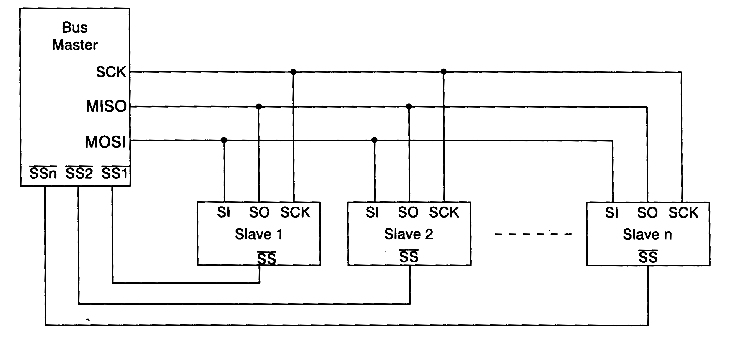
\includegraphics[width=15cm]{grafika/spi.jpg}
   \caption{SPI}
\end{figure}

Na magistrali występuje jeden układ nadrzędny - Master oraz co najmniej jeden Slave.
Master generuje zegar na linii SCK.
Master wysyła dane do Slavów szeregowo linią MOSI, Slavy odsyłają dane linią MISO. Transmisja jest fullduplexowana - przesył w obu kierunkach poszczególnych bitów następuje równocześnie w takt zegara.
Między układami współdzielone są linie zegara oraz danych. Odseparowane natomiast są linie CS poszczególnych slavów - wywołanie niskiego potencjału przez mastera aktywuje danego slava do uczestnictwa w wymianie danych.


\newpage
\subsubsection{Połączenia}

\begin{figure}[htb]
   \centering
   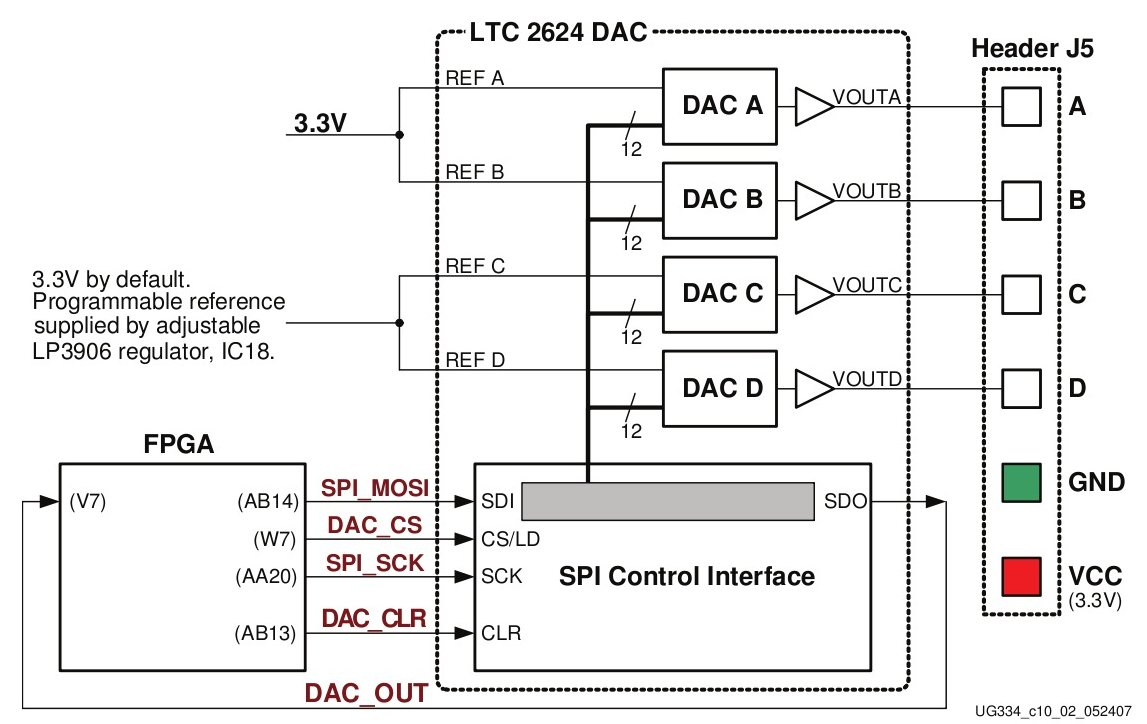
\includegraphics[width=15cm]{grafika/dac.jpg}
   \caption{Schemat polaczen ukladow LTC2624 i FPGA}
\end{figure}

Przed pierwszym użyciem należy układ zresetować chwilowo obniżając stan linii DAC\_CLR.

Na linie SPI\_SCK należy podać zegar o częstotliwości nie przekraczającej 50Mhz. Obniżając stan linii DAC\_CS rozpoczynamy komunikację z układem. Wtedy w takt zegara przesyłamy szeregowo do niego kolejne bity danych linią SPI\_MOSI. LTC2624 ładuje kolejne przesyłane bity do swojego rejestru przesuwnego na narastającym zboczu zegara oraz zwraca swoją poprzednią zawartość linią DAC\_OUT na opadającym zboczu. Natychmiast po wysłaniu kompletu danych należy koniecznie podnieść stan linii DAC\_CS zakańczając transmisję.

\begin{figure}[htb]
   \centering
   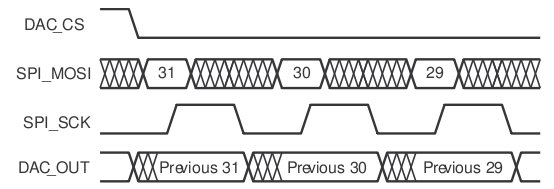
\includegraphics[width=15cm]{grafika/dac-waveform.jpg}
   \caption{Wykres stanow linii}
\end{figure}


\newpage
\subsubsection{Protokół komunikacji}

\begin{figure}[htb]
  \centering
	\begin{register}{H}{Przesylana ramka}{a}
	\label{dacprotocol}%
	\regfield{Nieistotne}{8}{24}{10000000}%
	\regfield{Komenda}{4}{20}{1100}%
	\regfield{Adres}{4}{16}{1111}%
	\regfield{Wartosc}{12}{4}{100000000000}%
	\regfield{Nieistotne}{4}{0}{0001}%
	\end{register}
\end{figure}

Dane przesyłane do układu LTC2624 są 32-bitową ramką uwidocznioną powyższym polem bitowym. Bity wysyła się kolejno zaczynając od najstarszego. Transmisja zaczyna się ośmioma nic nie znaczącymi bitami. Po nich wysyłane jest 4-bitowe pole komendy - typowo o wartości $0011$, co oznacza natychmiastowe wystawienie zadanej wartości napięcia. Następnie podawany jest adres konwertera według poniższej tabeli

\begin{figure}[htb]
  \centering
	\begin{tabular}{|c|c|c|c|l|}
	  \multicolumn{1}{r}{19}&\multicolumn{1}{r}{}&\multicolumn{1}{r}{}&\multicolumn{1}{r}{16}&\multicolumn{1}{l}{Adres}\\
		\hline
		0&0&0&0 & DAC A\\
		\hline
		0&0&0&1 & DAC B\\
		\hline
		0&0&1&0 & DAC C\\
		\hline
		0&0&1&1 & DAC D\\
		\hline
		1&1&1&1 & Wszystkie\\
		\hline
	\end{tabular}
\end{figure}

Trzecie pole jest 12-bitową wartością binarną odpowiadającą wystawianemu napięciu. Ramka kończy się 4 nieistotnymi bitami. W przykładzie na wszystkich konwerterach pojawiłaby się połowa z ustawionych zakresów napięć.


\subsection{Aplikacja}

Zrealizowany projekt wykorzystuje opisany układ obecny na płytce przetwornika cyfrowo-analogowego. Po wystartowaniu lub resecie ustawiane jest zerowe napięcie. Używając dwóch przycisków można napięcie podnieść lub obniżyć w zakresie $0V - 3.3V$ z krokiem $32 / 4096$. Zawsze pojedynczy pakiet ustawia wszystkie cztery konwertery dostępne w układzie na raz. Podgląd na bieżący stan podawanego napięcia pokazują diody LED.


\subsection{Synteza}

\subsubsection{Warstwa wierzchnia}

Moduł najwyższy łączy interfejs SPI przetworników z odfiltrowanymi z drgań sygnałami przycisków i diodami led. Instancjuje także moduł kontrolera i warstwę spajającą interfejs DAC-a z wewnętrznym SPI.
%% \begin{lstlisting}[label=Rs232Tx,caption=Rs232Tx.v,firstnumber=14]
\begin{lstlisting}[label=Top,caption=Top.v]
module Top (
   input CLK50MHZ,
   input RST,
   // dac
   output SPI_SCK,
   output DAC_CLR,
   output DAC_CS,
   output SPI_MOSI,
   input DAC_OUT,
   // control
   input BTN_WEST,
   input BTN_EAST,
   input BTN_NORTH,
   output [7:0] LED
);
\end{lstlisting}

\subsubsection{Kontroler}

Kontroler posiada połączenia do przycisków $RST$ i odfiltrowanych z drgań $less$, $more$ oraz $maxx$. W zależności od ich wciśnięć, kontroler wystawi nową wartość $data$ dostępną dla DAC-ów oraz zawiadamia o tym flagą $dactrig$. Zawsze adresowane są wszystkie DAC-i z komendą natychmiastowego ustawienia nowej wartości. Podgląd aktualnie wystawianej wartości pokazują diody LED.
\begin{lstlisting}[label=Controller,caption=Controller.v]
module Controller(
   input RST,
   input CLK50MHZ,
   // verilog module interface
   output     [11:0] data,
   output reg [3:0 ] address = 4'b1111,
   output reg [3:0 ] command = 4'b0011,
   output            dactrig,
   // control
   input             less,
   input             more,
   input             maxx,
   // leds
   output     [7:0 ] LED
);
\end{lstlisting}

Moduł ma wewnętrzny rejestr przechowujący bieżący stan wystawianego napięcia. Wciskane przyciski go modyfikują.
\begin{lstlisting}[label=Controller,caption=Controller.v,firstnumber=17]
   reg [7:0] d = 8'd0;
   always @(posedge CLK50MHZ)
      if(RST)       d <= 8'd0;
      else if(maxx) d <= 8'hff;
      else if(less) begin if( 0 < d ) d <= d - 1; end
      else if(more) begin if( ~&  d ) d <= d + 1; end

   assign data = { d, 4'h0 };
   assign LED = d;
\end{lstlisting}

Pojawienie się nowej wartości należy obwieścić modułowi nadrzędnemu.
\begin{lstlisting}[label=Controller,caption=Controller.v,firstnumber=27]
   assign dactrig = (less || more || maxx);
\end{lstlisting}

\subsubsection{DacSpi}
Jest to warstwa zajmująca się opóźnieniem zegara bazowego oraz doprecyzowaniem ogólnego modułu SPI. $50mHz$ to górna granica działania kostki DAC-ów. Dla pewniejszego działania, zalecane jest niższe taktowanie, co zrealizowane jest modułem $ClkMod$ z podanym parametrem dzielnika $DIV = 6$. Do SPI przekazane zostaje 32-bitowe połączenie spojone z danych uzyskanych od kontrolera i otoczone bitami nieznaczącymi.
\begin{lstlisting}[label=Controller,caption=Controller.v,firstnumber=32]
   wire [WIDTH-1:0] dacdatatosend = {8'h80, command, address, data, 4'h1};
\end{lstlisting}

Zegar magistrali SPI taktowany jest tylko w razie konieczności. Resetowanie DAC-ów następuje odwrotnie do przycisku reset.
\begin{lstlisting}[label=Controller,caption=Controller.v,firstnumber=51]
   assign SPI_SCK = (~dacdone) ? spi_sck : 1'b0;
   assign DAC_CLR = ~RST;
\end{lstlisting}


\subsection{Symulacja}

W teście inicjalizowane są zegar, reset, moduł syntezowalny, zachowawczy i przypadek testowy.

\subsubsection{Przypadek testowy}

W przypadku testowym powoływane są ustawiacze przycisków zwiększania oraz zmniejszania napięcia, a także monitor linii resetu. Symulacja czeka na zresetowanie układu, następnie poprzez przyciski dwukrotnie zwiększa napięcie i raz je zmniejsza.

\subsubsection{DAC zachowawczo}

Interfejs modułu ukazuje poziomy logowania wraz z liniami upozorowanej kostki.
\begin{lstlisting}[label=DacLTC2624Behav,caption=DacLTC2624Behav.v,firstnumber=0]
module DacLTC2624Behav
#(
   // LOGLEVEL = 0
   // 	bez zadnych komunikatow
   // LOGLEVEL = 1
   // 	pokazuje bledy
   // LOGLEVEL = 2
   // 	pokazuje ostrzezenia
   //
   // LOGLEVEL = 3
   // 	informuje o odbieraniu danych, odebraniu i ich interpretacji
   // LOGLEVEL = 4
   // 	informuje o wlasciwej liczbie bitow w pakiecie
   // LOGLEVEL = 5
   // 	informuje o adresie daca
   // LOGLEVEL = 6
   // 	informuje o zakonczeniu odbioru danych (moment podniesienia flagi DAC_CS)
   // LOGLEVEL = 7
   // 	informuje o odbieraniu poszczegolnych pol pakietu
   // LOGLEVEL = 8
   // 	informuje o odbiorze poszczegolnych bitow pakietu
   // LOGLEVEL = 9
   // 	informuje o przebiegu resetowania daca
   parameter LOGLEVEL      = 5,
   parameter LOGLEVEL_SCK  = 3,
   parameter LOGLEVEL_CLR  = 3,
   parameter LOGLEVEL_MOSI = 3,
   parameter LOGLEVEL_SCK_MOSI = 3
) (
   input  SPI_SCK,
   input  DAC_CS,
   input  DAC_CLR,
   input  SPI_MOSI,
   output DAC_OUT
);
\end{lstlisting}

Moduł zachowawczy sprawdza, czy użytkownik zresetował kostke przed użyciem. Informacja ta zawarta zostaje w rejestrze $inited$. Wątek powróci przy odebraniu ramki.
\begin{lstlisting}[label=DacLTC2624Behav,caption=DacLTC2624Behav.v,firstnumber=63]
   // Przed uzyciem daca nalezy go najpierw zresetowac poprzez chwilowe obnizenie linii DAC_CLR
   reg 	  inited = 1'b0;
   initial begin

      if(LOGLEVEL >= 9)
         $display("%t\t INFO9\t [ %m ] \t Oczekiwanie na zresetowanie daca", $time);
      monitor_clr.wait_for_low();
      monitor_clr.ensure_low_during( 40 );
      monitor_clr.wait_for_high();

      if(LOGLEVEL >= 9)
         $display("%t\t INFO9\t [ %m ] \t Zresetowano daca", $time);
      inited = 1'b1;
   end
\end{lstlisting}

Kalkulowany jest indeks przesyłanego bitu.
\begin{lstlisting}[label=DacLTC2624Behav,caption=DacLTC2624Behav.v,firstnumber=78]
   // Rejest zlicza kolejno odbierane bity
   reg [5:0] idx = 6'd0;
   // Licznik idx zerowany jest na poczatku kazdej transmisji
   always @(negedge DAC_CS)
      idx <= 6'd0;
   // Resetuj licznik lub go podbij na kazdym narastajacym zboczu zegara
   always @(posedge SPI_SCK) begin
      idx <= idx + 1;
   end
\end{lstlisting}

Zadanie odbioru pojedynczego bitu upewnia się, że wartość bitu jest stabilna w zczytywanym oknie czasowym.
\begin{lstlisting}[label=DacLTC2624Behav,caption=DacLTC2624Behav.v,firstnumber=88]
   // Odbiera jeden bit
   task receive_bit
   (
      output received_bit
   );
      begin
         if(LOGLEVEL >= 8)
            $display("%t\t INFO8\t [ %m ] \t Odbieranie kolejnego bitu", $time);

	 // Po wlaczeniu daca do szyny spi zegar powinien zaczac nisko
         monitor_sck.ensure_low_during( 40 );
         monitor_sck.wait_for_high();

	 // 4ns stabilnosci zegara i zczytywanej linii miso
	 monitor_sck_mosi.ensure_state_during( 4 );
	 received_bit = SPI_MOSI;

	 // konczenie okresu zegara
	 monitor_sck.ensure_high_during( 40 - 4 );
	 monitor_sck.wait_for_low();

         if(LOGLEVEL >= 8)
            $display("%t\t INFO8\t [ %m ] \t Odebrano bit %b", $time, received_bit);
      end
   endtask
\end{lstlisting}

Odbieranie całego pakietu podzielone jest na mniejsze fragmenty w celu dokładniejszego logowania komunikacji.
\begin{lstlisting}[label=DacLTC2624Behav,caption=DacLTC2624Behav.v,firstnumber=114]
   // Pola bitowe otrzymanych danych
   reg [ 3:0] dontcare4 = 4'd0;
   reg [11:0] value     = 12'd0;
   reg [ 3:0] address   = 4'd0;
   reg [ 3:0] command   = 4'd0;
   reg [ 8:0] dontcare8 = 8'd0;
   wire [31:0] packet = { dontcare4, value, address, command, dontcare8 };
   // Odbiera 32 bity danych pakietu
   task receive_packet
   ();
      integer i;
      begin
         if(LOGLEVEL >= 3)
            $display("%t\t INFO3\t [ %m ] \t Odbieranie pakietu", $time);

	 // Receive 8 dont care bits
         if(LOGLEVEL >= 7)
            $display("%t\t INFO7\t [ %m ] \t Odbieranie 8 pierwszych nie znaczacych bitow", $time);
	 for(i = 0; i < 8; i=i+1) begin
            receive_bit( dontcare8[i] );
	 end

	 // Receive command
         if(LOGLEVEL >= 7)
            $display("%t\t INFO7\t [ %m ] \t Odbieranie komendy", $time);
	 for(i = 0; i < 4; i=i+1) begin
            receive_bit( command[i] );
	 end

	 // Receive address of dac
         if(LOGLEVEL >= 7)
            $display("%t\t INFO7\t [ %m ] \t Odbieranie adresu", $time);
	 for(i = 0; i < 4; i=i+1) begin
            receive_bit( address[i] );
	 end

	 // Receive 12 bit of value
         if(LOGLEVEL >= 7)
            $display("%t\t INFO7\t [ %m ] \t Odbieranie wartosci", $time);
	 for(i = 0; i < 12; i=i+1) begin
            receive_bit( value[i] );
	 end

	 // Receive 4 dont care bits
         if(LOGLEVEL >= 7)
            $display("%t\t INFO7\t [ %m ] \t Odbieranie 4 ostatnich nie znaczacych bitow", $time);
	 for(i = 0; i < 4; i=i+1) begin
            receive_bit( dontcare4[i] );
	 end

         if(LOGLEVEL >= 3)
            $display("%t\t INFO3\t [ %m ] \t Odebrano pakiet", $time);
      end
   endtask
\end{lstlisting}

Obniżenie linii $DAC\_CS$ rozpoczyna przesył ramki. Tutaj potwierdzane jest uprzednie zresetowanie układu.
\begin{lstlisting}[label=DacLTC2624Behav,caption=DacLTC2624Behav.v,firstnumber=169]
   reg received_packet = 1'b0;
   // Odbiera pakiet i wyzwala o tym flage
   always @(negedge DAC_CS)
      if(!inited) begin
         if(LOGLEVEL >= 1)
            $display("%t\t BLAD\t [ %m ] \t Nie zresetowano ukladu przed nadaniem nadanych", $time);
      end else begin
         if(LOGLEVEL >= 3)
            $display("%t\t INFO3\t [ %m ] \t Odbieranie danych", $time);

	 received_packet = 1'b0;
	 receive_packet();
	 received_packet = 1'b1;

      end
\end{lstlisting}

Śledzić należy przesłanie zbyt dużej ilości bitów w ramce.
\begin{lstlisting}[label=DacLTC2624Behav,caption=DacLTC2624Behav.v,firstnumber=185]
   // Zatrzaskuje moment przeslania zbyt wielu bitow
   reg too_many_bits = 1'b0;
   always @(negedge DAC_CS)
      too_many_bits = 1'b0;
   always @(posedge received_packet) begin
      monitor_sck.wait_for_low();
      monitor_sck.wait_for_high();

      too_many_bits = 1'b1;
   end
   wire received_too_many_bits = received_packet && too_many_bits;
\end{lstlisting}

Podniesienie linii $DAC\_CS$ oznacza zakończenie nadawania ramki. Wypisywane są wtedy szczegółowe komunikaty o zaadresowanym DAC-u, podanej komendzie oraz wystawionej wartości, lub błędy transmisji jeśli jakiekolwiek zaistniały.
\begin{lstlisting}[label=DacLTC2624Behav,caption=DacLTC2624Behav.v,firstnumber=197]
   // Podniesienie DAC_CS konczy transmisje, weryfikowane i wypisywane sa przeslane dane
   always @(posedge DAC_CS) begin
      if(inited) begin

         // Zakomunikuj koniec odbioru
         if(LOGLEVEL >= 6)
            $display("%t\t INFO6\t [ %m ] \t Podniesiono flage DAC_CS, co konczy odbior danych", $time);

         //Bledy nieodpowiedniej ilosci odebranych bitow
         if(received_too_many_bits) begin
            if(LOGLEVEL >= 1)
               $display("%t\t BLAD\t [ %m ] \t Do daca wyslanych zostalo wiecej bitow niz 32", $time);
         end else if(idx < 32) begin
            if(LOGLEVEL >= 1)
               $display("%t\t BLAD\t [ %m ] \t Do daca wyslanych zostalo %d bitow. Nalezy wyslac 32", $time, idx);

         // Odebrano wlasciwa ilosc bitow, parsuj dane
         end else begin

            if(LOGLEVEL >= 4)
               $display("%t\t INFO4\t [ %m ] \t Odebrane dane zawieraja wlasciwa ilosc bitow", $time);

               // Wypisz odebrane pola
               if(LOGLEVEL >= 3)
                  $display("%t\t INFO3\t [ %m ] \t Ustawiono\twartosc %d (0x%h)\tna adresie %d (0x%h)\tz komenda %d (0x%h)", $time, value, value, address, address, command, command);

               // Wypisz ustawian-ego/-ne dac-a/-i bazujac na przeslanym adresie lub zakomunikuj blad
               case(address)
                  4'b0000:
                     if(LOGLEVEL >= 5)
                        $display("%t\t INFO5\t [ %m ] \t Dac o adresie %b (0x%h) jest dac-iem A", $time, address, address);
                  4'b0001:
                     if(LOGLEVEL >= 5)
                        $display("%t\t INFO5\t [ %m ] \t Dac o adresie %b (0x%h) jest dac-iem B", $time, address, address);
                  4'b0010:
                     if(LOGLEVEL >= 5)
                        $display("%t\t INFO5\t [ %m ] \t Dac o adresie %b (0x%h) jest dac-iem C (mozliwe ustawienie wzmocnienia)", $time, address, address);
                  4'b0011:
                     if(LOGLEVEL >= 5)
                        $display("%t\t INFO5\t [ %m ] \t Dac o adresie %b (0x%h) jest dac-iem D (mozliwe ustawienie wzmocnienia)", $time, address, address);
                  4'b1111:
                     if(LOGLEVEL >= 5)
                        $display("%t\t INFO5\t [ %m ] \t Dac o adresie %b (0x%h) odpowiada wszystkim dac-om", $time, address, address);
                  default:
                     if(LOGLEVEL >= 1)
                        $display("%t\t BLAD\t [ %m ] \t Nieprawidlowy adres daca", $time);
               endcase

               // Sprawdz czy wyslano wlasciwa komende, jedyna poprawna to 0011
               // Odbierana komenda jest w odwroconym porzadku bitow
               if(command != 4'b1100)
                  if(LOGLEVEL >= 1)
                     $display("%t\t BLAD\t [ %m ] \t Nieprawidlowa komenda %b (0x%h) - aby natychmiastowo ustawic dac nalezy wyslac 0011 (0x3)", $time, command, command);

         end
      end
   end
\end{lstlisting}

Istotnym aspektem modułu behawioralnego jest zwracanie poprzednio zapamiętanej wartości linią $DAC\_OUT$.
\begin{lstlisting}[label=DacLTC2624Behav,caption=DacLTC2624Behav.v,firstnumber=255]
   // Na linii wyjsciowej DAC_OUT beda sie pojawiac kolejne bity wypychane z rejestru przesuwnego daca
   // Nastepuje to na narastajacym zboczu zegara SPI_SCK przy obnizonej linii aktywacji transmisji DAC_CS
   assign DAC_OUT = DAC_CS ? 1'b0 : packet[31];
\end{lstlisting}

\subsubsection{Przebieg}

Przedstawiona symulacja pokazuje wykres przebiegów czasowych linii prowadzących do układu DAC. Pola z bitami nieistotnymi przesyłanej ramki są tak dobrane aby pojedynczymi, skrajnymi pikami pokazywały początek i koniec ramki.

\begin{figure}[htb]
   \centering
   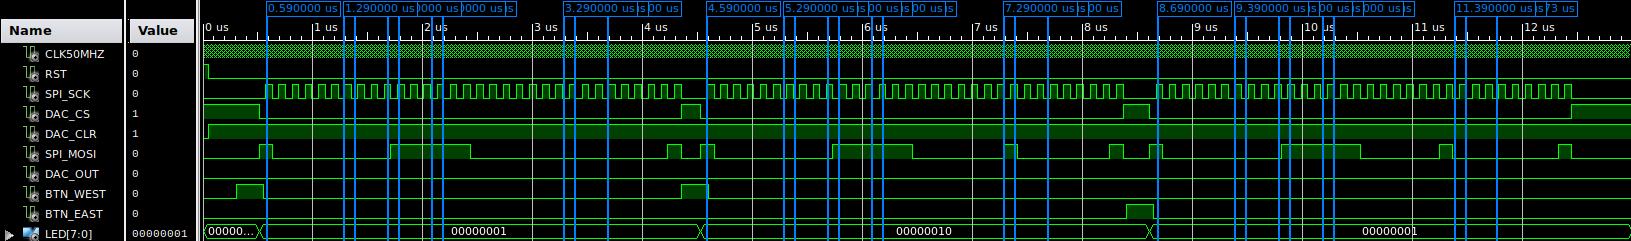
\includegraphics[width=15cm]{grafika/dac_sim.png}
\end{figure}

Zestaw komunikatów z przebiegu symulacji.
\begin{lstlisting}[label=dacout,caption=DAC logi]
  301000 INFO3 [ TopTest.TopTestBench_ ]  Zwiekszanie napiecia
  510000 INFO3 [ TopTest.DacLTC2624Behav_ ]  Odbieranie danych
  510000 INFO3 [ TopTest.DacLTC2624Behav_.receive_packet ]  Odbieranie pakietu
  4350000 INFO4 [ TopTest.DacLTC2624Behav_ ]  Odebrane dane zawieraja wlasciwa ilosc bitow
  4350000 INFO3 [ TopTest.DacLTC2624Behav_ ]  Ustawionowartosc    0 (0x000)na adresie 15 (0xf)z komenda 12 (0xc)
  4350000 INFO5 [ TopTest.DacLTC2624Behav_ ]  Dac o adresie 1111 (0xf) odpowiada wszystkim dac-om
  4351000 INFO3 [ TopTest.TopTestBench_ ]  Zwiekszanie napiecia
  4351000 INFO3 [ TopTest.DacLTC2624Behav_.receive_packet ]  Odebrano pakiet
  4530000 INFO3 [ TopTest.DacLTC2624Behav_ ]  Odbieranie danych
  4530000 INFO3 [ TopTest.DacLTC2624Behav_.receive_packet ]  Odbieranie pakietu
  8370000 INFO4 [ TopTest.DacLTC2624Behav_ ]  Odebrane dane zawieraja wlasciwa ilosc bitow
  8370000 INFO3 [ TopTest.DacLTC2624Behav_ ]  Ustawionowartosc  128 (0x080)na adresie 15 (0xf)z komenda 12 (0xc)
  8370000 INFO5 [ TopTest.DacLTC2624Behav_ ]  Dac o adresie 1111 (0xf) odpowiada wszystkim dac-om
  8371000 INFO3 [ TopTest.DacLTC2624Behav_.receive_packet ]  Odebrano pakiet
  8401000 INFO3 [ TopTest.TopTestBench_ ]  Zmniejszanie napiecia
  8610000 INFO3 [ TopTest.DacLTC2624Behav_ ]  Odbieranie danych
  8610000 INFO3 [ TopTest.DacLTC2624Behav_.receive_packet ]  Odbieranie pakietu
  12450000 INFO4 [ TopTest.DacLTC2624Behav_ ]  Odebrane dane zawieraja wlasciwa ilosc bitow
  12450000 INFO3 [ TopTest.DacLTC2624Behav_ ]  Ustawionowartosc   64 (0x040)na adresie 15 (0xf)z komenda 12 (0xc)
  12450000 INFO5 [ TopTest.DacLTC2624Behav_ ]  Dac o adresie 1111 (0xf) odpowiada wszystkim dac-om
  12451000 INFO3 [ TopTest.DacLTC2624Behav_.receive_packet ]  Odebrano pakiet
\end{lstlisting}


\newpage
\section{Rotor}

Płytka Spartan 3AN jest wyposażona w obrotowy przełącznik o dwóch wyprowadzeniach do FPGA. W stanie jałowym są one przyłączone do wysokiego potencjału. Mechaniczne obracanie pokrętła powoduje zwieranie styków na liniach i uziemienie napięcia. Kierunek obrotu wyznacza linia, która wcześniej zostanie zwarta do masy lub, co jest ekwiwalentne, wcześniej wróci do stanu jałowego.

\begin{figure}[htb]
   \centering
   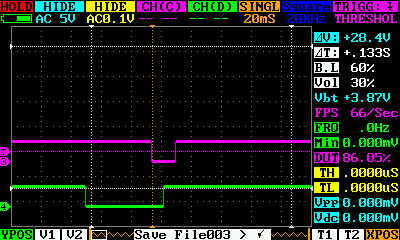
\includegraphics[width=13cm]{grafika/dso/rotor-w-prawo-jeden.png}
   \caption{Obrót w kierunku zgodnym z ruchem wskazówek zegara. Fioletowa linia pokazuje sygnał $rota$, natomiast zielona $rotb$.}
\end{figure}

\begin{figure}[htb]
   \centering
   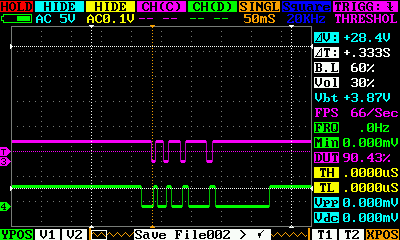
\includegraphics[width=13cm]{grafika/dso/rotor-w-prawo-wiele.png}
   \caption{Kilka obrotów następujących po sobie}
\end{figure}

\subsection{Aplikacja}

FPGA po skonfigurowaniu lub zresetowaniu zapala jedną diode, piątą lub szóstą w szeregu. Obrót rotora powoduje przesunięcie stanu wszystkich diód o jedną pozycję w lewo lub w prawo w zależności od kierunku obrotu. Pozycje skrajne się cyklicznie uzupełniają. Rotor można także nacisnąć, co spowoduje zmianę stanu pierwszej diody na przeciwny. Nacisk ma własną linię sygnałową nie powiązaną z obrotowymi.

\subsection{Synteza}

\subsubsection{Warstwa wierzchnia}

FPGA korzysta z wyprowadzeń zegara, dolnego przycisku resetu, $ROT\_CENTER$ jest do obsługi wciśnięć. $ROT\_A$ oraz $ROT\_B$ są połączeniami do pokrętła. Są też wyprowadzenia dla diód i dodatkowe połączenia pokrętła na oscyloskop.
\begin{lstlisting}[label=Rs232Tx,caption=Rs232Tx.v,firstnumber=14]
module Top (
    input        CLK50MHZ,
    input        RST,
    // rotor control
    input        ROT_CENTER,
    input        ROT_A,
    input        ROT_B,
    // leds
    output [7:0] LED,
    // debug
    output       DEBUG_A,
    output       DEBUG_B
    );
\end{lstlisting}
Przycisk $ROT\_CENTER$ jest pozbawiany drgań styków dzięki przeprowadzeniu przez $Debouncer$-a. Zainstancjonowane są tu także moduły $Rotor$-a oraz $Controller$-a. Wyprowadzenia debugera to przypisania ciągłe na odpowiadające połączenia obrotu.

\subsubsection{Rotor}
$Rotor$ otrzymuje bezpośrednio sygnały o mechanicznych obrotach pokrętła i je interpretuje, w wyniku czego sygnalizuje wykryte obroty wraz z ich rozpoznanym kierunkiem.
\begin{lstlisting}[label=Rotor,caption=Rotor.v]
module Rotor(
    input clk,
    input rst,
    // inputs
    input rota,
    input rotb,
    // one pulse output direction signals
    output left,
    output right
);
\end{lstlisting}

Dla zobrazowanie dalszych zależności między sygnałami, zamieszczony jest zrzut z symulacji.
\begin{figure}[htb]
   \centering
   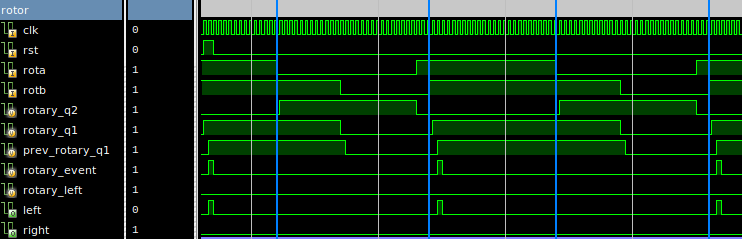
\includegraphics[width=15cm]{grafika/rotor.png}
   \caption{Symulacja sygnałów rotora}
\end{figure}

Rejestry pomocnicze zatrzaskują stan linii $rotb$. $rotary\_q1$ gdy wyprowadzenia pokrętła są zgodne, natomiast $rotary\_q2$ gdy są przeciwne.
\begin{lstlisting}[label=Rotor,caption=Rotor.v,firstnumber=12]
    reg rotary_q1 = 1'b0;
    always @(posedge clk)
        if(rota ~^ rotb)
            rotary_q1 <= rotb;

    reg rotary_q2 = 1'b0;
    always @(posedge clk)
        if(rota ^ rotb)
             rotary_q2 <= rotb;
\end{lstlisting}

Dodatkowy rejestr $prev\_rotary\_q1$ przechowuje wartość $rotary\_q1$ z poprzedniej chwili. To umożliwia wykrycie zbocza narastającego $rotary\_q1$, czyli momentu gdy obrót się skończył i oba wyprowadzenia pokrętła są ponownie wysokie w stanie jałowym.

Pogląd na kierunek obrotu daje drugi rejestr pomocniczy $rotary\_q2$. Linie pokrętła nie kończą wysterowywania obrotu jednocześnie. Kolejność powrotów mówi o kierunku obrotu. $rotary\_q2$ zachowa stan $rotb$ w chwili pierwszego powrotu. Wystarczy teraz sprawdzić zachowany stan $rotary\_q2$, by odpowiedzieć czy ona wróciła pierwsza, co implikowałoby obrót w prawo - zgodny z ruchem wskazówek zegara.
\begin{lstlisting}[label=Rotor,caption=Rotor.v,firstnumber=22]
    reg prev_rotary_q1 = 1'b0;
    reg rotary_event = 1'b0;
    reg rotary_left = 1'b0;
    always @(posedge clk) begin
        prev_rotary_q1 <= rotary_q1;
        if(~prev_rotary_q1 && rotary_q1) begin
            rotary_event <= 1'b1;
            rotary_left <= rotary_q2;
        end else
            rotary_event <= 1'b0;
    end

    assign left = rotary_event & ~rotary_left;
    assign right = rotary_event & rotary_left;

endmodule
\end{lstlisting}

\subsubsection{Kontroler}

Kontroler operuje na rejestrze, który powiązany jest z diodami led na płytce. Po świeżej konfiguracji płytki świeci się dioda piąta. Przycisk resetu ustawia jedynie szóstą. Przycisk centralny pokrętła zmieni stan diody pierwszej na przeciwny. Kontroler dostaje też impulsy $left$ oraz $right$ informujący o zajściu obrotu i jego kierunku. Wtedy przesuwa bity rejestru w wyznaczonym kursie.
\begin{lstlisting}[label=Controller,caption=Controller.v]
module Controller(
         input clk,
         input rst,
         // tick inputs
         input center,
         input left,
         input right,
         //  leds
         output reg [7:0] leds = 8'b0001_0000
    );

    always @(posedge clk)
        if(rst)           leds <= 8'b0010_0000;
        else if(center)   leds[0] <= ~leds[0];
        else if(left)     leds <= { leds[6:0], leds[7] };
        else if(right)    leds <= { leds[0], leds[7:1] };

endmodule
\end{lstlisting}

\subsection{Symulacja}
Moduły testowe jedynie symulują obracanie pokrętła przez użytkownika poprzez wysterowanie jego sygnałów. Moduł najwyższy symulacji jedynie zapewnia zainstancjonowanie zegara, resetu, modułu syntezowalnego i testowego odpowiednika pokrętła.

\subsubsection{Przypadek testowy}


\begin{lstlisting}[label=TopTestBench,caption=TopTestBench.v]
module TopTestBench #(
   LOGLEVEL = 3,
   LOGLEVEL_BEHAV = 3,
   LOGLEVEL_BEHAV_CENTER = 3,
   LOGLEVEL_BEHAV_ROTA = 3,
   LOGLEVEL_BEHAV_ROTB = 3
) (
   // rotor control
   output ROT_CENTER,
   output ROT_A,
   output ROT_B
);
\end{lstlisting}
On z kolei instancjuje $Rotor\_behav$ i operuje pokrętłem poprzez jego zestaw zadań.
\begin{lstlisting}[label=TopTestBench,caption=TopTestBench.v,firstnumber=37]
      // kilka ruchow
      rotor_behav.turn_left();
      rotor_behav.turn_left();
      rotor_behav.press_center();
      rotor_behav.turn_right();
\end{lstlisting}

\subsubsection{Rotor zachowawczo}

Rotor dysponuje garstką prostych zadań.
\begin{lstlisting}[label=Rotor_behav,caption=Rotor\_behav.v]
   task turn_left();
      begin
         ..
         // rozpoczecie skretu w lewo
         set_rota.low_during( 250 );
         set_rotb.low_during( 300 );

         // konczenie skretu w lewo
         set_rota.high_during( 50 );
         set_rotb.high_during( 500 );
         ..
      end
   endtask
\end{lstlisting}

Obrót w prawo jest analogiczny do lewego.
\begin{lstlisting}[label=Rotor_behav,caption=Rotor\_behav.v]
   task turn_right();
      begin
         ..
         // rozpoczecie skretu w prawo
         set_rotb.low_during( 250 );
         set_rota.low_during( 300 );

         // konczenie skretu w prawo
         set_rotb.high_during( 50 );
         set_rota.high_during( 500 );
         ..
      end
   endtask
\end{lstlisting}


Po zwolnieniu wciśniętego przycisku, dołożona jest chwila przerwy.
\begin{lstlisting}[label=Rotor_behav,caption=Rotor\_behav.v]
   task press_center();
      begin
         ..
         set_center.high_during( 400 );
         set_center.low_during( 200 );
         ..
      end
   endtask
\end{lstlisting}

\subsubsection{Komunikaty}

Przedstawione jest pełne wyjście z pierwszego zadania obrotu w lewo przy maksymalnym stopniu logowania.

\begin{lstlisting}
Time resolution is 1 ps
Simulator is doing circuit initialization process.
     0 INFO3 [ TopTest.TopTestBench_.rotor_behav.set_center.state ]  Stan sygnalow zostanie zmieniony. Obecny stan 'x' (0x x), spodziewany stan '0' (0x 0)
     0 INFO4 [ TopTest.TopTestBench_.rotor_behav.set_center.state ]  Stan sygnalow zostal zmieniony. Obecny stan '0' (0x 0)
     0 INFO3 [ TopTest.TopTestBench_.rotor_behav.set_rota.state ]  Stan sygnalow zostanie zmieniony. Obecny stan 'x' (0x x), spodziewany stan '1' (0x 1)
     0 INFO4 [ TopTest.TopTestBench_.rotor_behav.set_rota.state ]  Stan sygnalow zostal zmieniony. Obecny stan '1' (0x 1)
     0 INFO3 [ TopTest.TopTestBench_.rotor_behav.set_rotb.state ]  Stan sygnalow zostanie zmieniony. Obecny stan 'x' (0x x), spodziewany stan '1' (0x 1)
Finished circuit initialization process.
300000 INFO3 [ TopTest.TopTestBench_ ]  Poczatek symulacji
300000 INFO3 [ TopTest.TopTestBench_.rotor_behav.turn_left ]  Obracanie pokretla w lewo
300000 INFO3 [ TopTest.TopTestBench_.rotor_behav.set_rota.state ]  Stan sygnalow zostanie zmieniony. Obecny stan '1' (0x 1), spodziewany stan '0' (0x 0)
300000 INFO4 [ TopTest.TopTestBench_.rotor_behav.set_rota.state ]  Stan sygnalow zostal zmieniony. Obecny stan '0' (0x 0)
300000 INFO5 [ TopTest.TopTestBench_.rotor_behav.set_rota.state_during ]  Sygnal w stanie 0 (hex 0) zostaje zamrozony przez zadany okres czasu        250
550000 INFO6 [ TopTest.TopTestBench_.rotor_behav.set_rota.state_during ]  Przeczekiwanie stanu 0 (hex 0) zostalo zakonczone po        250
550000 INFO3 [ TopTest.TopTestBench_.rotor_behav.set_rotb.state ]  Stan sygnalow zostanie zmieniony. Obecny stan '1' (0x 1), spodziewany stan '0' (0x 0)
850000 INFO3 [ TopTest.TopTestBench_.rotor_behav.set_rota.state ]  Stan sygnalow zostanie zmieniony. Obecny stan '0' (0x 0), spodziewany stan '1' (0x 1)
850000 INFO4 [ TopTest.TopTestBench_.rotor_behav.set_rota.state ]  Stan sygnalow zostal zmieniony. Obecny stan '1' (0x 1)
850000 INFO5 [ TopTest.TopTestBench_.rotor_behav.set_rota.state_during ]  Sygnal w stanie 1 (hex 1) zostaje zamrozony przez zadany okres czasu         50
900000 INFO6 [ TopTest.TopTestBench_.rotor_behav.set_rota.state_during ]  Przeczekiwanie stanu 1 (hex 1) zostalo zakonczone po         50
900000 INFO3 [ TopTest.TopTestBench_.rotor_behav.set_rotb.state ]  Stan sygnalow zostanie zmieniony. Obecny stan '0' (0x 0), spodziewany stan '1' (0x 1)
400000 INFO4 [ TopTest.TopTestBench_.rotor_behav.turn_left ]  Obrocono pokretlo w lewo
\end{lstlisting}


\newpage
\section{Rs232}

Rs232 jest asynchronicznym, szeregowym standardem komunikacyjnym. Zdefiniowane są osobne linie do wysyłanych i odbieranych danych. Szybkość transmisji ustala się ręcznie w urządzeniach końcowych.

Stanem wysokim określony jest stan bezczynności. Nadawanie danych rozpoczyna się od opuszczenia linii $tx$ na okres jednego bitu tzw. startowego. Następnie przesyłane są kolejne bity danych i kończone są wysokim bitem stopu. Standard przewiduje możliwy bit parzystości poprzedzający stop.

\subsection{Aplikacja}
Zaimplementowana aplikacja oczekuje wysłania bajtu danych przez urządzenie po drugiej stronie kabla, po czym mu go odsyła w niezmienionej postaci. Działa jak zwykłe echo. Pracuje z prędkością 115200 bitów na sekundę. Nie implementuje bitu parzystości.

\subsection{Synteza}

\subsubsection{Warstwa wierzchnia}
Moduł najwyższy w zasadzie przepuszcza wszystkie połączenia do właściwego modułu echa. Jedynie wyprowadza dodatkowo stan linii komunikacyjnych na złącze oscyloskopu do łatwej analizy. Natomiast moduł echa instancjuje część odbierającą i transmitującą dane oraz je łączy.
\lstinputlisting[caption=Rs232Echo.v]{../projects/rs232/Rs232Echo.v}


\subsubsection{Transmisja}
Transmiter jest prostszy, zatem od niego warto zacząć. Należy przekazać mu w parametrach taktowanie zegara podstawowego płytki oraz zakładaną prędkość pracy. Aby z modułu skorzystać wystarczy podsunąć wysyłany bajt połączeniem $TxD\_data$, po czym podnieść na jeden cykl $TxD\_start$. Wtedy zacznie formować stan linii wyjściowej $TxD$ poprzez serializację dostarczonego bajtu wraz z dodatkowymi skrajnymi bitami startu i stopu. Swoją zajętość sygnalizuje flagą $TxD\_busy$.
\begin{lstlisting}[label=Rs232Tx,caption=Rs232Tx.v]
module Rs232Tx
#(
   parameter FREQ = 50000000,   // 50MHz
   parameter BAUD = 115200      // 115 200 bounds/sec
) (
   input       CLK50MHZ,
   input       RST,
   input       TxD_start,
   input [7:0] TxD_data,
   output      TxD,
   output      TxD_busy
);
\end{lstlisting}

Zalecany standard 232 przewiduje tolerancję niedokładności zegara nie przekraczającą $5\%$ w dowolnym kierunku. Przy przesyłanych łącznie 10 bitach w pakiecie oznacza to rozjechanie się zegarów odbiornika i nadajnika maksymalnie o pół bitu. Prosty licznik oparty na zegarze podstawowym $50Mhz$ nie spełnia wymagań. Należy zachowywać resztę z dodawań po każdym przepełnieniu. Dlatego do wyznaczenia momentu nadania kolejnego bitu służy dedykowany moduł $BaudRateGenerator$ z wykalkulowaną inkrementacją.
\begin{lstlisting}[label=Rs232Tx,caption=Rs232Tx.v,firstnumber=14]
   `include "../../generic/log2.v"
   localparam N = log2(BAUD);

   wire        BaudTick;
   wire        TxD_ready;
   BaudRateGenerator #(
        .INC( ((BAUD<<(N-4))+(FREQ>>5))/(FREQ>>4) ), // = 302
        .N(N)
     ) baud115200 (
        .CLK50MHZ(CLK50MHZ),
        .RST(RST),
        .en(TxD_busy),
        .tick(BaudTick)
    );
\end{lstlisting}

Znany moduł do serializacji zajmuje się wysyłaniem danych w takt sygnału generowanego przez $BaudRateGenerator$. Dane te należy otoczyć bitem startu i stopu oraz w całości zanegować dla spójności z jałową jedynką.
\begin{lstlisting}[label=Rs232Tx,caption=Rs232Tx.v,firstnumber=29]
    // START BIT, data, STOP BIT
    wire [9:0]  rs_data = { 1'b1, ~TxD_data, 1'b0 };
   // output TxD line should be high at idle
    wire        TxD_neg;
    Serial #(
        .WIDTH(10)
    ) Serial_ (
        .CLKB(CLK50MHZ),
        .RST(RST),
        // serial module interface
        .rx(1'b0),
        .tx(TxD_neg),
        .data_in(rs_data),
        .trig(TxD_start),
        .ready(TxD_ready),
        .tick(BaudTick)
    );

   assign TxD      = ~ TxD_neg;
   assign TxD_busy = ~ TxD_ready;

endmodule
\end{lstlisting}


\subsubsection{Odbiór}
Moduł odbiorczy podobnie ma parametryzowane zegar podstawowy płytki oraz szybkość pracy. Gdy odbierze nowe dane, wystawia je na wyjścia $RxD\_data$ oraz informuje o zdarzeniu flagą $RxD\_data\_ready$ przez jeden cykl.
\begin{lstlisting}[label=Rs232Rx,caption=Rs232Rx.v]
module Rs232Rx
#(
        parameter FREQ = 50000000,      // 50MHz
        parameter BAUD = 115200         // 115 200 bounds/sec
) (
        input        CLK50MHZ,
        input        RST,
        input        RxD,
        output [7:0] RxD_data,
        output       RxD_data_ready
);
\end{lstlisting}

Protokół jest asynchroniczny, więc sygnał zegarowy nie jest przekazywany, co utrudnia nieco odbiór. Linia $RxD$ jest próbkowana z trzykrotnie większą częstotliwością, a przyjęty odebrany bit jest wynikiem głosowania próbek. Podejście wymusza powołanie również szybszego modułu $BaudRateGenerator$-a.
\begin{lstlisting}[label=Rs232Rx,caption=Rs232Rx.v,firstnumber=13]
   `include "../../generic/log2.v"
   localparam N = log2(BAUD);

   wire              receving;
   wire              BaudTick3;
   BaudRateGenerator #(
        // 3 times oversampling
        .INC( ((BAUD*3<<(N-7))+(FREQ>>8))/(FREQ>>7) ), // = 2416
        .N(N)
    ) baud_115200x3 (
        .CLK50MHZ(CLK50MHZ),
        .RST(RST),
        .en(receving),
        .tick(BaudTick3)
    );

    wire        BaudTick;
    BaudRateGenerator #(
        .INC( ((BAUD<<(N-4))+(FREQ>>5))/(FREQ>>4) ), // = 302
        .N(N)
    ) baud_115200 (
        .CLK50MHZ(CLK50MHZ),
        .RST(RST),
        .en(receving),
        .tick(BaudTick)
    );
\end{lstlisting}

Tutaj instancjalizowany jest rejestr przesuwny dla próbek oraz kreowany układ głosujący przypisaniem ciągłym.
\begin{lstlisting}[label=Rs232Rx,caption=Rs232Rx.v,firstnumber=40]
   wire [2:0]   rx3;
   Shiftreg #(
      .WIDTH(3)
   ) rx3_shitftreg (
           .CLKB(CLK50MHZ),
           .en(1'b1),
           .set(1'b0),
           .tick(BaudTick3),
           .rx(RxD),
           .data_in(3'b000),
           .data_out(rx3)
           );

   // Vote for rx value
   wire                    rx =
                           rx3 != 3'b000 &&
                           rx3 != 3'b001 &&
                           rx3 != 3'b010 &&
                           rx3 != 3'b100;
\end{lstlisting}

Serializer zajmuje się deserializacją napływających bitów pakietu. Bity początkowy startu i końcowy stopu zostają obcięte.
\begin{lstlisting}[label=Rs232Rx,caption=Rs232Rx.v,firstnumber=59]
   wire                    trig;
   wire                    ready;
   wire [9:0]              data_out;
   Serial #(
        .WIDTH(10)
    ) Serial_ (
        .CLKB(CLK50MHZ),
        .RST(RST),
        // serial module interface
        .rx(rx),
        .data_in(10'b0),
        .data_out(data_out),
        .trig(trig),
        .ready(ready),
        .tick(BaudTick)
    );

   // get rid of START and STOP bits
   assign RxD_data = data_out[8:1];
\end{lstlisting}

Konieczna jest maszyna stanów. Najpierw wyczekuje niskiego bitu startu, po czym odbiera pakiet i zgłasza jego przyjęcie. Cykl się powtarza.
\begin{lstlisting}[label=Rs232Rx,caption=Rs232Rx.v,firstnumber=79]
   localparam [1:0]
     WAIT_STARTBIT = 3'd0,
     START_RECEVING = 3'd1,
     RECEVING = 3'd2,
     RECEIVED = 3'd3;

   reg [2:0]               state = WAIT_STARTBIT;
   always @(posedge CLK50MHZ)
     if(RST)
       state <= WAIT_STARTBIT;
     else
       case(state)
         WAIT_STARTBIT:
           if(~RxD)
             state <= START_RECEVING;
         START_RECEVING:
             state <= RECEVING;
         RECEVING:
           if(ready)
             state <= RECEIVED;
         RECEIVED:
             state <= WAIT_STARTBIT;
       endcase

   assign       trig = (state == START_RECEVING);
   assign       RxD_data_ready = (state == RECEIVED);
   assign       receving = (state == RECEVING);

endmodule
\end{lstlisting}

\subsection{Symulacja}

Moduł symulacyjny wysyła serię bajtów wzorcowych, po czym oczekuje odesłania ich z powrotem.

Moduł najwyższy $TopTest$ kreuje instancje zegara, resetu, $Rs232$ i wierzchni moduł syntezowalny oraz zapewnia między nimi połączenia.


\subsubsection{Rs232}


$Rs232$ zawiera pamięć z napisem, który zamierza nadać, po czym odebrać.
\begin{lstlisting}[label=sim/Rs232,caption=sim/Rs232.v,firstnumber=28]
   localparam CHARS = 8;
   reg [7:0] mem [CHARS:0];
   initial begin
      mem[0] = "A";
      mem[1] = "G";
      mem[2] = "H";
      mem[3] = " ";
      mem[4] = "W";
      mem[5] = "F";
      mem[6] = "i";
      mem[7] = "I";
      mem[8] = "S";
   end
\end{lstlisting}

Nadawane są kolejno litery korzystając z zadania modułu zachowawczego.
\begin{lstlisting}[label=sim/Rs232,caption=sim/Rs232.v,firstnumber=42]
   integer j = 0;
   initial begin
      ..
      // wyslanie kolejnych liter napisu powitalnego
      for(j=0; j<CHARS; j=j+1) begin
         rs232_behav.transmit( mem[j] );
         ..
      end
   end
\end{lstlisting}

Śledzona jest linia $rx$, która to powinny wysłane dane otrzymać z powrotem w tej samej formie i porządku, co zostaje poddane weryfikacji.
\begin{lstlisting}[label=sim/Rs232,caption=sim/Rs232.v,firstnumber=64]
   integer k = 0;
   reg [7:0] byte_received = 8'd0;
   always @(negedge rx) begin
      if(inited) begin

         // odbior bajtu
         rs232_behav.receive( byte_received );
         ..

         // weryfikacja
         if( byte_received != mem[k] )
            if(LOGLEVEL >= 1)
               $display("%t\t ERROR [ %m ] \t Odebrany bajt %b 0x%h %d %s rozni sie od wyslanego wzorca %b 0x%h %d %s", $time, byte_received, byte_received, byte_received, byte_received, mem[k], mem[k], mem[k], mem[k]);

         // inkrementuj numer biezacego bajtu
         k = k + 1;
     end
  end
\end{lstlisting}


\subsubsection{Rs232 zachowawczo}

Moduł udostępnia zadania do wysyłania oraz odbierania danych. Zajmuje się formowanie ich w pakiety z doklejonymi bitami startu i stopu lub wyłuskiwaniem jego zawartości. Informuje o przebiegu swojej pracy z wybraną sześciostopniową dokładnością poziomu logowania.
\begin{lstlisting}[label=sim/Rs232 behav,caption=sim/Rs232 behav.v]
module Rs232_behav
#(
   // LOGLEVEL = 0
   //      bez zadnych komunikatow
   // LOGLEVEL = 1
   //      pokazuje bledy
   // LOGLEVEL = 2
   //      pokazuje ostrzezenia
   //
   // LOGLEVEL = 3
   //      informuje o wyslaniu/otrzymaniu pelnego bajtu
   // LOGLEVEL = 4
   //      informuje o wysylaniu/otrzymywaniu poszczegolnych bitow
   // LOGLEVEL = 5
   //      informuje o wyslaniu/otrzymywaniue start i stop bitow
   // LOGLEVEL = 6
   //      informuje o przeczekiwaniu tolerowanego przesuniecia zegara
   parameter LOGLEVEL=3,
   parameter LOGLEVEL_RX=3,
   parameter LOGLEVEL_TX=3,

   parameter BAUDRATE = 115_200
) (
   input rx,
   output tx
);
\end{lstlisting}

Wyliczone są czasy trwania pojedynczego bitu na podstawie żądanej prędkości transmisji oraz tolerancji na błąd przesunięcia zegara.
\begin{lstlisting}[label=sim/Rs232 behav,caption=sim/Rs232 behav.v,firstnumber=64]
   // czas jednego okresu przy zakladanej szybkosci
   localparam PERIOD = 1_000_000_000 / BAUDRATE;
   // tolerancja zegara
   localparam BITTOL = 0.05 * PERIOD;
\end{lstlisting}

Zadanie wysyłające przyjmuje bajt danych. Wysyła go w pętli poprzedzając bitem startu i zakańczając stopem.
\begin{lstlisting}[label=sim/Rs232 behav,caption=sim/Rs232 behav.v,firstnumber=64]
   // Zadanie wysyla przekazany bajt wraz z poprzedajacym bitem startu i nastepujacym stopu
   task transmit
   (
      input [7:0] byte_tosend
   );
      integer     i;
      begin
         ..
         set_tx.low_during( PERIOD );

         // Przekazany bajt
         for(i=0; i < 8; i=i+1) begin
            set_tx.state_during( PERIOD, byte_tosend[i] );
            ..
         end

         // Stop bit
         ..
         set_tx.high_during( PERIOD );
         ..
      end
   endtask
\end{lstlisting}

Zadanie odbierające dane symetrycznie do nadającego spodziewa się bitu startu, bajtu danych i stop bitu.
\begin{lstlisting}[label=sim/Rs232 behav,caption=sim/Rs232 behav.v,firstnumber=118]
   task receive
   (
      output reg [7:0] byte_received
   );
      integer i;
      reg startbit;
      reg stopbit;
      begin
         // Zaczekaj na start bit
         ..
         monitor_rx.wait_for_low();
         ..
         // Odbierz bit startu
         receive_bit( startbit );
         if(startbit != 1'b0)
            if(LOGLEVEL >= 1)
               $display("%t\t ERROR [ %m ] \t Bit startu powinien byc niski", $time);
         ..
         // Odbierz bajt danych
         for(i=0; i < 8; i=i+1) begin
            receive_bit( byte_received[i] );
            ..
         end

         // Odbierz oczekiwany stop bit
         ..
         receive_bit( stopbit );
         if(stopbit != 1'b1)
            if(LOGLEVEL >= 1)
               $display("%t\t ERROR [ %m ] \t Oczekiwany bit stopu powinien byc wysoki", $time);
         ..
      end
   endtask
\end{lstlisting}

Odbiór bitu realizowany jest w kolejnym dedykowanym zadaniu. Sprawdzane jest, czy linia $rx$ jest stabilna przez długość trwania okresu z wyłączeniem początkowego i końcowego możliwego błędu synchronizacji zegarów.
\begin{lstlisting}[label=sim/Rs232 behav,caption=sim/Rs232 behav.v,firstnumber=89]
   // Zadanie odbiera bit probkujac go 3 krotnie
   task receive_bit
   (
      output reg received
   );
      begin
         ..
         #(BITTOL);
         ..
         monitor_rx.ensure_same_during( (PERIOD-2*BITTOL) );
         ..
         received = rx;
         ..
         #(BITTOL);
         ..
      end
   endtask
\end{lstlisting}


\subsubsection{Wyjście}

\begin{lstlisting}[label=rsout,caption=Rs log,firstnumber=255]
96800000 INFO3 [ TopTest.rs232 ]  Wyslano bajt '01001000' (0x 48) (dec  72) (ascii H)
183600000 INFO3 [ TopTest.rs232 ]  Wyslano bajt '01000101' (0x 45) (dec  69) (ascii E)
183710000 INFO3 [ TopTest.rs232 ]  Odebrano bajt '01001000' (0x 48) (dec  72) (ascii H)
270400000 INFO3 [ TopTest.rs232 ]  Wyslano bajt '01001100' (0x 4c) (dec  76) (ascii L)
270570000 INFO3 [ TopTest.rs232 ]  Odebrano bajt '01000101' (0x 45) (dec  69) (ascii E)
\end{lstlisting}

%% \subsubsection{HDL}
%% \lstinputlisting[caption=Top.v]{../projects/rs232/Top.v}
%% \lstinputlisting[label=Rs232Tx,caption=Rs232Tx.v]{../projects/rs232/Rs232Tx.v}
%% \lstinputlisting[label=Rs232Rx,caption=Rs232Rx.v]{../projects/rs232/Rs232Rx.v}

%% 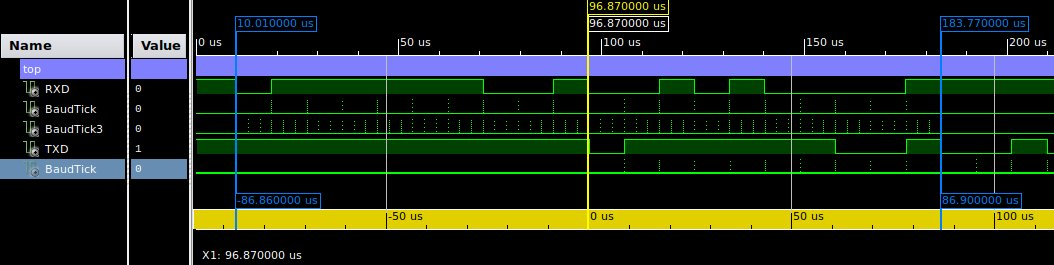
\includegraphics[width=15cm]{grafika/rs232-waveform.jpg}

%% \subsubsection{HDL}
%% \lstinputlisting[caption=Top.v]{../projects/rs232/sim/Rs232_behav.v}

\newpage
\section{Klawiatura PS2}

\subsection{Interfejs PS2}

Interfejs PS2 występuje najczęściej jako 6 stykowe gniazdo mini-DIN, takie też dostępne jest na płytce Spartan 3AN Starter Kit. Złącze mini-DIN ustandaryzowane zostało przez niemiecki instytut Deutsches Institut fuer Norm http://www.din.de, natomiast sposób komunikacji opracowała firma IBM w 1987 roku.

\begin{figure}[htb]
   \centering
   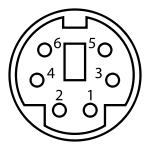
\includegraphics[width=2cm]{grafika/150px-MiniDIN-6_Connector_Pinout.png}
   \caption{Port mini-DIN}
\end{figure}

Styk trzeci jest masą, styk czwarty zasila urządzenia peryferyjne napięciem 5 V podając natężenie nie większe niż 275mA. Linią pierwszą wymieniane są dane w takt zegara na linii piątej. Tyle wystarcza do komunikacji z urządzeniem peryferyjnym myszki lub klawiatury. Połączenia numer dwa i sześć zazwyczaj nie są wykorzystywane. Jednak w rzadkich przypadkach producent może je wykorzystać dla drugiego urządzenia. Wtedy z pomocą kabla rozdzielającego można podłączyć mysz i klawiaturę do jednego, wspólnego gniazda mini-DIN. To rozwiązanie stosowane jest w starych laptopach oraz na płytce Spartan 3AN dla oszczędności miejsca.

Linie zegara i danych wysterowane są wysoko w stanie jałowym. Obie są dwukierunkowe, co jest zrealizowane przez konfigurację otwartego kolektora podciągniętego do stanu wysokiego. Zegar taktowany jest zawsze przez urządzenie peryferyjne z częstotliwością w zakresie $10 - 16.7 kHz$. Urządzenie przesyłając porcje danych do hosta najpierw przesyła niski bit startu, po czym następuje bajt danych w kolejności zaczynającej od bitu najmniej znaczącego, dalej jest bit parzystości i wysoki bit stopu. Stan bitów może być zmieniany w połowie czasu wysokiego zegara, bity odczytywane są przez hosta na zboczu opadającym.

Host może wysłać komendę do urządzenia. Przetrzymuje on wtedy linie zegarową oraz danych w stanach niskich przez czas co najmniej 100ms. Po tym zwalnia linie zegarową. Jest do żądanie do urządzenia o umożliwienie przesłania danych i wytaktowanie linii zegarowej. Po podaniu zegara, host ustawia bity w chwilach niskiego zegara. Ramka wygląda podobnie zawierając bit startu, bajt danych, parzystość i stop. Jednak po tym następuje dodatkowy bit potwierdzenia. Jest to obniżenie linii danych przez urządzenie i wygenerowania dla niego dodatkowego pulsu zegara. Potwierdza to właściwy odbiór danej.

\subsection{Klawiatura}

Klawiatura PS2 nadaje momenty wciśnięcia lub zwolnienia poszczególnych klawiszy. Jeśli klawisz jest przetrzymany dłużej, wtedy nadawane są przypomnienia jego wciśnięcia w odstępach 100ms.

Kody wciskanych klawiszy, nazywane skan kodami, powiązane są z ich położeniem i wcale się nie zakłada układu QWERTY rozmieszczenia klawiszy. Skan kody wymagają przekonwertowania do odpowiadającego użytkownikowi układu znaków.

Skan kod zajmuje jeden bajt. Krótkie wciśnięcie klawisza wysyła jego skan kod w pojedynczej ramce komunikacyjnej. Zwolnienie klawisza jest zdefiniowane przez wysłanie ramki poprzedzającej z bajtem F0 i kolejnej ramki ze skan kodem klawisza zwalnianego.

Rozróżnia się klawisze lewego oraz prawego alt-a i cntr-la. Lewe klawisze przesyłane są jak wszystkie pozostałe. Natomiast klawisze prawe poprzedzone są ramką o treści E0.

Do klawiatury można wysyłać polecenia od hosta. Polecenie echo określone bajtem $EE$ powoduje odesłanie przez klawiaturę tego samego bajtu $EE$. Można ustawić częstotliwość powtarzania wciśniętego klawisze komendą $F3$. Po niej klawiatura odpowiada potwierdzeniem $FA$ i następny bajt przesyła host z żądaną częstotliwością. Komenda $ED$ ustawia stan diod led $Caps Lock$, $Scroll Lock$, $Num Lock$. Klawiatura ją także potwierdza odsyłając $FA$ i oczekuje kolejnego bajtu z maską diod.

\subsection{Aplikacja}

Aplikacja odbiera przesłany przez klawiaturę bajt i wyświetla go na diodach led. Można zauważyć skan kod wciskanego klawisza oraz mignięcia bajtu F0 przy zwalnianiu. Aplikacja nie przesyła do klawiatury żadnych komend.

\subsection{Synteza}

\subsubsection{Warstwa wierzchnia}
Moduł najwyższy jedynie instancjuje kontrolera i moduł klawiatury.
\begin{lstlisting}[label=Top,caption=Top.v]
module Top (
    input  CLK50MHZ,
    input  RST,
    // keyboard
    input  PS2_CLK1,
    input  PS2_DATA1,
    output [7:0] LED,
);

    wire [7:0] scancode;
    wire scan_ready;
    Keyboard keyboard_ (
        .CLK50MHZ(CLK50MHZ),
        .RST(RST),
        .ps2_clk(PS2_CLK1),
        .ps2_data(PS2_DATA1),
        .scancode(scancode),
        .scan_ready(scan_ready)
    );

    Controller controller_ (
        .CLK50MHZ(CLK50MHZ),
        .RST(RST),
        .scancode(scancode),
        .scan_ready(scan_ready),
        .led(LED)
    );

endmodule
\end{lstlisting}

\subsubsection{Kontroler}
Kontroler jedynie wyświetla na diodach przesłany skan kod.
\begin{lstlisting}[label=Controller,caption=Controller.v]
module Controller(
  input 	   CLK50MHZ,
  input 	   RST,
  input [7:0] 	   scancode,
  input 	   scan_ready,
  output reg [7:0] led = 8'b0011_1100
);

    always @(posedge CLK50MHZ)
        if(RST)
          led <= 8'b0111_1110;
        else if( scan_ready )
          led <= scancode;

endmodule
\end{lstlisting}

\subsubsection{Klawiatura}
Najważniejszym modułem projektu jest sama klawiatura. Przyjmuje linie zegarową $ps2\_clk$ i danych $ps2\_data$, po odebraniu skan kodu wystawia go przewodem równoległym $scancode$ i informuje o tym ustawiając flagę $scan\_ready$.
\begin{lstlisting}[label=Keyboard,caption=Keyboard.v]
module Keyboard(
    input  CLK50MHZ,
    input  RST,
    input  ps2_clk,
    input  ps2_data,
    output [7:0] scancode,
    output scan_ready
    );
\end{lstlisting}

Wykrywanie zbocza opadającego zegara zrealizowane jest dwubitowym rejestrem przesuwnym i ciągłym porównywaniem go z wzorcem zbocza w pomocniczym module $Bits\_Reverse$.
\begin{lstlisting}[label=Keyboard,caption=Keyboard.v,firstnumber=10]
   // Detect negative edge on input ps2 clock line
   wire    ps2_clk_negedge;
   Edge_Detector ps2_clk_negedge_detector (
      .clk(CLK50MHZ),
      .signal(ps2_clk),
      .neg(ps2_clk_negedge)
   );
\end{lstlisting}

Przesyłana ramka zczytywana jest szeregowo na wykrytym zboczu opadającym przy wykorzystaniu modułu serializacji. Moduł odbiera jedynie 10 pierwszych bitów z ramki, ostatni stop bit nie jest zapisywany. Ponieważ pierwszy takt zegara ps2 wprawia maszynę stanów w ruch i dopiero włącza serializację do pracy, takt ten nie zostanie policzony wewnątrz serializacji. Obejściem byłoby dopisanie rejestru opóźniającego takty zegara ps2 o cykl i przekazanie go do serializacji lub, co jest prostsze, obcięcie ramki.
\begin{lstlisting}[label=Keyboard,caption=Keyboard.v,firstnumber=18]
   wire        trig;
   wire        ready;
   wire [9:0] frame;
   Serial #(
      // ignore 11th stop bit as first tick is not counted
      .WIDTH(10)
   ) Serial_ (
      .CLKB(CLK50MHZ),
      .RST(RST),
      // serial module interface
      .rx(ps2_data),
      .data_in(10'b0),
      .data_out(frame),
      .trig(trig),
      .ready(ready),
      .tick(ps2_clk_negedge)
   );
\end{lstlisting}

Ramka pozbawiana jest otaczających bitów startu, parzystości i stopu, co ekstrahuje przesyłany bajt danych. Ogólny moduł do obsługi rejestru przesuwnego zaprojektowany został do odbioru bitów w kolejności od najbardziej znaczącego. Protokół PS2 przesyła je w odwrotnej kolejności, przez co wymagane jest użycie dodatkowego modułu przywracającego pierwotny porządek. Odebrane dane nie są weryfikowane pod kątem zgodności z bitem parzystości.
\begin{lstlisting}[label=Keyboard,caption=Keyboard.v,firstnumber=36]
   // Get rid of start and odd bits, then reverse bit order of the data
   Bits_Reverse reversing (
      .orginal( frame[9:2] ),
      .reversed( scancode)
   );
\end{lstlisting}

Klawiatura zawiera maszynę stanów. Najpierw czeka na rozpoczęcie transmisji opadającym zboczem zegara. Kiedy to nastąpi, uruchamia odbiór szeregowy i czeka na jego zakończenie. Zakończenie odbioru wprawia ją w ostatni stan sygnalizujący modułowi wyższemu gotowość odebranego bajtu.
\begin{lstlisting}[label=Keyboard,caption=Keyboard.v,firstnumber=42]
   localparam [2:0]
    WAIT_STARTBIT = 3'd0,
    START_RECEVING = 3'd1,
    RECEIVING = 3'd2,
    RECEIVED = 3'd3;

   reg [1:0]  state = WAIT_STARTBIT;
   always @(posedge CLK50MHZ)
     if(RST)
       state <= WAIT_STARTBIT;
     else
       case(state)
         WAIT_STARTBIT:
           if(ps2_clk_negedge)
             state <= START_RECEVING;
         START_RECEVING:
             state <= RECEIVING;
         RECEIVING:
           if(ready)
             state <= RECEIVED;
         RECEIVED:
             state <= WAIT_STARTBIT;
       endcase

    assign       trig = (state == START_RECEVING);
    assign       scan_ready = (state == RECEIVED);

endmodule
\end{lstlisting}


\subsection{Symulacja}

Moduł najwyższy $TopTest$ powołuje zegar, reset, moduł najwyższy syntezowalny oraz przypadek testowy do przeprowadzenia.

\subsubsection{Przypadek testowy}

Przypadek testowy powołuje instancję zachowawczą klawiatury, po czym operuje na jej zestawie zadań wciskając oraz zwalniając parę z nich.
\begin{lstlisting}[label=TopTestBench,caption=TopTestBench.v]
module TopTestBench (
    input RST,
    // keyboard
    output PS2_CLK1,
    output PS2_DATA1
);

   Keyboard_behav #(
      .LOGLEVEL(5)
   ) keyboard_behav (
      .clk(PS2_CLK1),
      .data(PS2_DATA1)
   );

   initial begin
      @(negedge RST);
      #10_000;

      keyboard_behav.press_right_alt();
      keyboard_behav.type_char("a");
      keyboard_behav.release_right_alt();

      keyboard_behav.type_(keyboard_behav.ENTER);
   end

endmodule
\end{lstlisting}

\subsubsection{Klawiatura zachowawczo}

Moduł zachowawczy przyjmuje parametr żądanej szczegółowości logowania oraz wysterowywuje linie zegara i danych.

\begin{lstlisting}[label=Keyboard_behav,caption=Keyboard\_behav.v]
module Keyboard_behav
#(
   // LOGLEVEL = 0
   //      bez zadnych komunikatow
   // LOGLEVEL = 1
   //      pokazuje bledy
   // LOGLEVEL = 2
   //      pokazuje ostrzezenia
   //
   // LOGLEVEL = 3
   //      informuje o wyslaniu/otrzymaniu pelnego bajtu
   // LOGLEVEL = 4
   //      informuje o wysylaniu/otrzymywaniu poszczegolnych bitow
   // LOGLEVEL = 5
   //      informuje o wyslaniu/otrzymywaniue start i stop bitow
   // LOGLEVEL = 6
   //      informuje o przeczekiwaniu tolerowanego przesuniecia zegara
   //
   parameter LOGLEVEL=3,
   parameter LOGLEVEL_CLK=3,
   parameter LOGLEVEL_DATA=3
) (
   output  clk,
   output  data
);
\end{lstlisting}

Ustawiane zostają stałe połowy okresu $HALF\_PERIOD = 7 000 000$ oraz ćwiartka. Instancjalizowane zostają moduły ustawiania linii zegara i danych oraz inicjalizowane zostają stanami wysokimi.

Konstrukcja zadania wysyłającego daną $send\_$ jest bliźniaczo podobna do zadania $transmit$ z modułu $Rs232\_behav$. Wysyłane bity są jedynie zmieniane w połowie wysokiego zegara, a ramka poszerzona jest o bit parzystości wyrażany operatorem redukcji
\begin{lstlisting}[label=Keyboard_behav,caption=Keyboard\_behav.v,firstnumber=75]
	 odd = ~^ scancode;
\end{lstlisting}

Zapisane są mapowania klawiszy specjalnych do odpowiadających skan kodów.
\begin{lstlisting}[label=Keyboard_behav,caption=Keyboard\_behav.v,firstnumber=110]
   // Pare klawiszy specjalnych

   reg [7:0] ESC         = 8'h76;
   reg [7:0] TAB         = 8'h0d;
   reg [7:0] BKSPC       = 8'h0d;
   reg [7:0] ENTER       = 8'h5a;
   reg [7:0] SPACE       = 8'h29;
   reg [7:0] LEFT_SHIFT  = 8'h12;
   reg [7:0] RIGHT_SHIFT = 8'h59;
   reg [7:0] LEFT_CTRL   = 8'h14;
   reg [7:0] LEFT_ALT    = 8'h11;

   reg [7:0] EXT         = 8'he0;
   reg [7:0] RELEASE     = 8'hf0;
\end{lstlisting}

Zdefiniowanych jest parę podstawowych operacji na klawiszach.
\begin{lstlisting}[label=Keyboard_behav,caption=Keyboard\_behav.v,firstnumber=125]
   // Zadania ogolne do wcisniecia, puszczenia oraz przetrzymania zadanego klawisza

   task press_
   (
      input [7:0] scancode
   );
      begin
         send_(scancode);
      end
   endtask

   task release_
   (
      input [7:0] scancode
   );
      begin
         press_(EXT);
	 press_(scancode);
      end
   endtask

   task type_
   (
      input [7:0] scancode
   );
      begin
	 press_(scancode);
	 #1000;
	 release_(scancode);
	 #1000;
      end
   endtask
\end{lstlisting}

Dla rozróżnienia lewego lub prawego ctrl-a, dołączone są dedykowane zadania. To samo podejście zastosowane jest dla alt-a.
\begin{lstlisting}[label=Keyboard_behav,caption=Keyboard\_behav.v,firstnumber=158]
   // Klawisze lewego i prawego alt-a oraz ctrl-a sa rozroznialne

   task press_left_control
   ();
      begin
	 press_(LEFT_CTRL);
      end
   endtask

   task release_left_control
   ();
      begin
	 release_(LEFT_CTRL);
      end
   endtask

   task press_right_control
   ();
      begin
	 press_(EXT);
	 press_(LEFT_CTRL);
      end
   endtask

   task release_right_control
   ();
      begin
	 press_(EXT);
	 release_(LEFT_CTRL);
      end
   endtask
\end{lstlisting}

Translacją znaków tablicy ASCII do odpowiadających skan kodów zajmuje się tablica $char_to_scancode$.
\begin{lstlisting}[label=Keyboard_behav,caption=Keyboard\_behav.v,firstnumber=220]
   // Mapowanie znaku do skan kodu
   reg [7:0] char_to_scancode [255:0];
   initial begin
       char_to_scancode["a"] = 8'h1c;
       char_to_scancode["b"] = 8'h32;
       ...
\end{lstlisting}

Ostatnie zadania operują na przekazanych znakach tablicy ASCII i przesyłają ich skan kod.
\begin{lstlisting}[label=Keyboard_behav,caption=Keyboard\_behav.v,firstnumber=262]
   // Zadania operuja na znakach

   task press_char
   (
      input [7:0] char
   );
      begin
         press_(char_to_scancode[char]);
      end
   endtask

   task release_char
   (
      input [7:0] char
   );
      begin
         release_(char_to_scancode[char]);
      end
   endtask

   task type_char
   (
      input [7:0] char
   );
      begin
         type_(char_to_scancode[char]);
      end
   endtask
\end{lstlisting}


\subsubsection{Przebieg}


Wycinek zrzutu ekranu pokazuje przebieg symulacji. Niebieskie markery oddzielają sekwencję dla poszczególnych klawiszy.
\begin{figure}[htb]
   \centering
   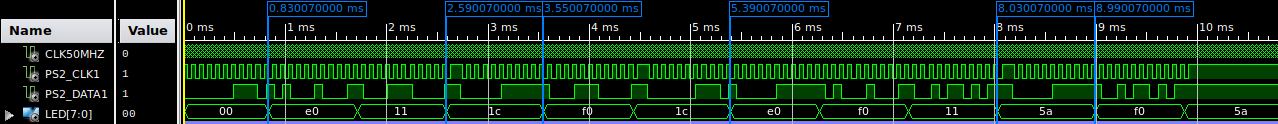
\includegraphics[width=15cm]{grafika/keyboard_sim.png}
   \caption{Przebieg symulacji}
\end{figure}


Zamieszczone jest wyjście logów dla domyślnych poziomów logowania.
\begin{lstlisting}[label=Keyboard_output,caption=Keyboard logs output]
  10000000 INFO3 [ TopTest.TopTestBench_.keyboard_behav.press_right_alt ]  Wcisnieto prawy alt
  10000000 INFO4 [ TopTest.TopTestBench_.keyboard_behav.press_ ]  Wcisnieto przycisk o skan kodzie 11100000 (0x e0)
  10000000 INFO5 [ TopTest.TopTestBench_.keyboard_behav.send_ ]  Wysylanie bajtu '11100000' (0x e0)
  890000000 INFO5 [ TopTest.TopTestBench_.keyboard_behav.send_ ]  Wyslano bajt 11100000 (0x e0)
  890000000 INFO4 [ TopTest.TopTestBench_.keyboard_behav.press_ ]  Wcisnieto przycisk o skan kodzie 00010001 (0x 11)
  890000000 INFO5 [ TopTest.TopTestBench_.keyboard_behav.send_ ]  Wysylanie bajtu '00010001' (0x 11)
  1770000000 INFO5 [ TopTest.TopTestBench_.keyboard_behav.send_ ]  Wyslano bajt 00010001 (0x 11)
  1770000000 INFO3 [ TopTest.TopTestBench_.keyboard_behav.type_char ]  Wpisywanie klawisza o literze/cyfrze 01100001 (0x 61) (dec  97) (ascii a)
  1770000000 INFO4 [ TopTest.TopTestBench_.keyboard_behav.type_ ]  Wpisywanie przycisku o skan kodzie 00011100 (0x 1c)
  1770000000 INFO4 [ TopTest.TopTestBench_.keyboard_behav.press_ ]  Wcisnieto przycisk o skan kodzie 00011100 (0x 1c)
  1770000000 INFO5 [ TopTest.TopTestBench_.keyboard_behav.send_ ]  Wysylanie bajtu '00011100' (0x 1c)
  2650000000 INFO5 [ TopTest.TopTestBench_.keyboard_behav.send_ ]  Wyslano bajt 00011100 (0x 1c)
  2730000000 INFO4 [ TopTest.TopTestBench_.keyboard_behav.release_ ]  Zwalnianie przycisku o skan kodzie 00011100 (0x 1c)
  2730000000 INFO4 [ TopTest.TopTestBench_.keyboard_behav.press_ ]  Wcisnieto przycisk o skan kodzie 11110000 (0x f0)
  2730000000 INFO5 [ TopTest.TopTestBench_.keyboard_behav.send_ ]  Wysylanie bajtu '11110000' (0x f0)
  3610000000 INFO5 [ TopTest.TopTestBench_.keyboard_behav.send_ ]  Wyslano bajt 11110000 (0x f0)
  3610000000 INFO4 [ TopTest.TopTestBench_.keyboard_behav.press_ ]  Wcisnieto przycisk o skan kodzie 00011100 (0x 1c)
  3610000000 INFO5 [ TopTest.TopTestBench_.keyboard_behav.send_ ]  Wysylanie bajtu '00011100' (0x 1c)
  4490000000 INFO5 [ TopTest.TopTestBench_.keyboard_behav.send_ ]  Wyslano bajt 00011100 (0x 1c)
  4570000000 INFO3 [ TopTest.TopTestBench_.keyboard_behav.release_right_alt ]  Zwalnianie prawego alt-a
  4570000000 INFO4 [ TopTest.TopTestBench_.keyboard_behav.press_ ]  Wcisnieto przycisk o skan kodzie 11100000 (0x e0)
  4570000000 INFO5 [ TopTest.TopTestBench_.keyboard_behav.send_ ]  Wysylanie bajtu '11100000' (0x e0)
  5450000000 INFO5 [ TopTest.TopTestBench_.keyboard_behav.send_ ]  Wyslano bajt 11100000 (0x e0)
  5450000000 INFO4 [ TopTest.TopTestBench_.keyboard_behav.release_ ]  Zwalnianie przycisku o skan kodzie 00010001 (0x 11)
  5450000000 INFO4 [ TopTest.TopTestBench_.keyboard_behav.press_ ]  Wcisnieto przycisk o skan kodzie 11110000 (0x f0)
  5450000000 INFO5 [ TopTest.TopTestBench_.keyboard_behav.send_ ]  Wysylanie bajtu '11110000' (0x f0)
  6330000000 INFO5 [ TopTest.TopTestBench_.keyboard_behav.send_ ]  Wyslano bajt 11110000 (0x f0)
  6330000000 INFO4 [ TopTest.TopTestBench_.keyboard_behav.press_ ]  Wcisnieto przycisk o skan kodzie 00010001 (0x 11)
  6330000000 INFO5 [ TopTest.TopTestBench_.keyboard_behav.send_ ]  Wysylanie bajtu '00010001' (0x 11)
  7210000000 INFO5 [ TopTest.TopTestBench_.keyboard_behav.send_ ]  Wyslano bajt 00010001 (0x 11)
  7210000000 INFO4 [ TopTest.TopTestBench_.keyboard_behav.type_ ]  Wpisywanie przycisku o skan kodzie 01011010 (0x 5a)
  7210000000 INFO4 [ TopTest.TopTestBench_.keyboard_behav.press_ ]  Wcisnieto przycisk o skan kodzie 01011010 (0x 5a)
  7210000000 INFO5 [ TopTest.TopTestBench_.keyboard_behav.send_ ]  Wysylanie bajtu '01011010' (0x 5a)
  8090000000 INFO5 [ TopTest.TopTestBench_.keyboard_behav.send_ ]  Wyslano bajt 01011010 (0x 5a)
  8170000000 INFO4 [ TopTest.TopTestBench_.keyboard_behav.release_ ]  Zwalnianie przycisku o skan kodzie 01011010 (0x 5a)
  8170000000 INFO4 [ TopTest.TopTestBench_.keyboard_behav.press_ ]  Wcisnieto przycisk o skan kodzie 11110000 (0x f0)
  8170000000 INFO5 [ TopTest.TopTestBench_.keyboard_behav.send_ ]  Wysylanie bajtu '11110000' (0x f0)
  9050000000 INFO5 [ TopTest.TopTestBench_.keyboard_behav.send_ ]  Wyslano bajt 11110000 (0x f0)
  9050000000 INFO4 [ TopTest.TopTestBench_.keyboard_behav.press_ ]  Wcisnieto przycisk o skan kodzie 01011010 (0x 5a)
  9050000000 INFO5 [ TopTest.TopTestBench_.keyboard_behav.send_ ]  Wysylanie bajtu '01011010' (0x 5a)
  9930000000 INFO5 [ TopTest.TopTestBench_.keyboard_behav.send_ ]  Wyslano bajt 01011010 (0x 5a)
\end{lstlisting}


\newpage
\section{VGA}
Standard VGA odpowiada za przesłanie obrazu do wyświetlacza. Wprowadziła go firma IBM w 1987 roku w jej linii komputerów osobistych. Standard definiuje maksymalne wymiary obrazu w trybie znakowym jako 720x480, natomiast w trybie  graficznym jest to 640x480 przy 16 lub 256 dostępnych kolorach i częstotliwości odświeżania do 70 Hz. Punkty obrazu, zwane pikselami, przesyłane są w porządku od lewej do prawej kolumny, zaczynając od górnego do dolnego wiersza.

Po przesłaniu każdego wiersza, następuje chwilowe obniżenie linii synchronizacyjnej $HSYNC$. Natomiast po przesłaniu całej ramki, chwilowo opuszczana jest linia $VSYNC$. W punktach tych i ich pewnym otoczeniu należy uziemić linie kolorów.

Kolor pikseli określa złożenie nasycenia trzech podstawowych barw: czerwonej, zielonej i niebieskiej. Ich stan podawany jest osobnymi liniami analogowo wartościami napięcia z zakresu $0.0V - 0.7V$.

Płytka Spartan wykorzystuje po 4 cyfrowe wyjścia FPGA dla każdej z barw łączone w drabinki rezystorowe tworząc proste ADC.

\subsection{Aplikacja}
Zaprojektowana aplikacja pokazuje na ekranie przyłączonego wyświetlacza jeden z ośmiu kolorów. Użytkownik wybiera ulubiony kolor posługując się dwoma przyciskami. Jeden z nich przełącza kolor tła na następną dostępną barwę, drugi wraca do poprzedniej. Końce listy dostępnych barw są połączone, próba wykroczenia poza nią powoduje płynne przejście na jej przeciwny koniec.

\subsection{Synteza}

\subsubsection{Połączenia}
\iffalse
\subsubsection{Top}
\fi
Moduł najwyższy przyjmuje sygnały zegarowy, resetu oraz dwóch przycisków służących zmianie koloru wyświetlanego tła. Moduł wyprowadza sygnały synchronizacji ramek i kolumn oraz pożądany kolor podany poprzez trzy czterobitowe rejestry nasycenia czerwieni, błękitu i zieleni.

\begin{lstlisting}[label=Topvga,caption=Top.v]
module Top (
    input        CLK50MHZ,
    input        RST,
    // vga interface
    output [3:0] VGA_R,
    output [3:0] VGA_G,
    output [3:0] VGA_B,
    output       VGA_HSYNC,
    output       VGA_VSYNC,
    // color control
    input        BTN_NEXT,
    input        BTN_PREV,
);
\end{lstlisting}

Sygnały przycisków przewijania należy pozbawić drgań styków wykorzystując poznany moduł $Debouncer$. Następnie zostają zainstancjonowane moduły $Sync$ służący synchronizacji oraz $Controller$, który obsługuje przyciski i podaje wybrany kolor.

\subsubsection{Synchronizacja}
Standard VGA powstał w czasach monitorów kineskopowych. Technologia ta ukierunkowywuje elektromagnesami naładowaną wiązkę o wybranej energii w punkt na luminoforze, czym wyzwala fotony światła. Momenty gdy wiązka powraca na początek kolejnej linii lub całej ramki są punktami synchronizacji. Podczas powrotów wiązki, a także w chwilach przed i po, musi być ona wygaszona (przez obniżenie wartości składowych kolorów), aby nie zakłócić kolorów nadanych luminoforowi w pierwszym przebiegu.

Zadaniem modułu synchronizacyjnego jest właściwe wytaktowanie linii zawiadamiających o początku nowej ramki lub nowej kolumny. Są to sygnały cyfrowe utrzymywane w stanie wysokim, w chwilach synchronizacji zostają obniżane. Domyślne parametry dostosowane są do przesyłania obrazu rozmiaru 640x480 pikseli przy częstotliwości odświeżania 60 Hz. Odmierzanie czasu przesyłu kolumn  bazuje na podstawowym zegarze występującym na płytce o częstotliwości 50 mHz. Natomiast przesłanie ramki sygnalizowane jest po zliczeniu wysłania odpowiedniej liczby kolumn.

Sygnał $dispalying$ określa czy kolory mogą być podawane, sygnały współrzędnych $x$ i $y$ podają bieżącą lokalizuję wiązki.

\begin{lstlisting}[label=Syncvga,caption=Sync.v]
module Sync
#(
   parameter H_S  = 2*800,
   parameter H_FP = 2*16,
   parameter H_PW = 2*96,
   parameter H_BP = 2*48,
   parameter V_S  = 521,
   parameter V_PW = 2,
   parameter V_FP = 10,
   parameter V_BP = 29
) (
   input         CLK50MHZ,
   input         RST,
   // vga interface
   output        VGA_HSYNC,
   output        VGA_VSYNC,
   // tick for next pixel
   output [10:0] x,
   output [10:0] y,
   output        displaying
);
\end{lstlisting}

Synchronizacja opiera się na dwóch licznikach. Pierwszy zlicza zegar podstawowy 50 mHz, drugi zlicza przepełnienia pierwszego śledząc bieżącą linie w ramce. Połączenia $i$ oraz $j$ są aktualnymi stanami liczników.
\begin{lstlisting}[label=Syncvga,caption=Sync.v,firstnumber=23]
        wire [10:0] i;
        wire        h;
        Counter #(
                .MAX(H_S)
        ) Counter_h (
                .CLKB(CLK50MHZ),
                // counter
                .en(1'b1),
                .rst(RST),
                .sig(1'b1), // count all CLK50MHZ ticks
                .cnt(i),
                .full(h)
        );

        wire [9:0] j;
        Counter #(
                .MAX(V_S)
        ) Counter_v (
                .CLKB(CLK50MHZ),
                // counter
                .en(1'b1),
                .rst(RST),
                .sig(h), // count h sync
                .cnt(j)
        );
\end{lstlisting}

Dzięki przypisaniu ciągłemu do warunku logicznego, liczniki w stanach od 0 do długości trwania pulsu wywołują efekt synchronizacji. Natomiast połączenie $dispalying$ obejmuje również chwile zakazu wyświetlania wokół tych punktów.
\begin{lstlisting}[label=Syncvga,caption=Sync.v,firstnumber=49]
        assign displaying = (
            i >= H_PW + H_BP &&
            i <  H_S  - H_FP &&
            j >= V_PW + V_BP &&
            j <= V_S  - V_FP
        );

        assign VGA_HSYNC = (i >  H_PW);
        assign VGA_VSYNC = (j >= V_PW);

        assign x = i - H_PW - H_BP;
        assign y = j - V_PW - V_BP;

endmodule
\end{lstlisting}

\subsubsection{Controller}

Moduł kontrolera odpowiada za kolory poszczególnych pikseli. Dostaje on informacje czy może podawać kolor oraz obecne położenie wiązki. Jednakże jest on uproszczony i wypełnia cały obszar jednym jedynie kolorem, a więc  położenie wiązki jest mu zupełnie zbędne. Dostępnych jest jedynie 8 kolorów. Kolory przełączane są dwoma przyciskami na następny lub poprzedni.
\begin{lstlisting}[label=Syncvga,caption=Sync.v,firstnumber=49]
module Controller (
    input      CLK50MHZ,
    input      RST,
    // vga interface
    output [3:0] VGA_R,
    output [3:0] VGA_G,
    output [3:0] VGA_B,
    // color control
    input        next,
    input        prev,
    input [10:0] x,
    input [10:0] y,
    input displaying
);
\end{lstlisting}

Kolor bieżący zapisany jest w trzybitowym rejestrze. Zmieniany jest poprzez zewnętrzne przyciski. Przepełnianie licznika zachowuje się jak wybieranie od początku.
\begin{lstlisting}[label=Syncvga,caption=Sync.v,firstnumber=16]
   reg [2:0]      i = 1;
   always @(posedge CLK50MHZ)
      if(RST)
        i <= 1;
      else if(next)
        i <= i + 1;
      else if(prev)
        i <= i - 1;
\end{lstlisting}

Każdy z bitów bieżącego koloru odpowiada jednej ze składowych podstawowych. Wartości pośrednie nie są wykorzystywane.
\begin{lstlisting}[label=Syncvga,caption=Sync.v,firstnumber=25]
    assign VGA_R = (displaying && i[0]) ? 4'hf : 4'h0;
    assign VGA_G = (displaying && i[1]) ? 4'hf : 4'h0;
    assign VGA_B = (displaying && i[2]) ? 4'hf : 4'h0;
\end{lstlisting}

\subsection{Symulacja}
Symulacja musi zweryfikować, czy sygnały synchronizacyjne pojawiają się w spodziewanych okresach oraz czy wtedy oraz w ich otoczeniu wiązka jest wygaszona. Do tego zliczane są linie w ramce.

\subsubsection{Przypadek testowy}
Zaimplementowana jest symulacja wciśnięć przycisków zmian kolorów. Wciskany jest dwukrotnie przycisk żądania następnego koloru, po czym raz wciśnięty zostaje przycisk koloru poprzedniego.

\subsubsection{Moduł behawioralny}
Za odbiór i sprawdzenie nadawanych sygnałów wtyczki VGA odpowiada moduł $Vga\_Behav$. Przyjmuje trzy czterobitowe sygnały kolorów oraz dwie synchronizujące linii i ramek. Moduł jedynie odbiera sygnały, nie generuje żadnych zwrotnych.

$Vga\_Behav$ przyjmuje szereg parametrów. Domyślne wartości odpowiadają odbiorowi obrazu o rozmiarach 640x480 pikseli przy częstotliwości odświeżania 60 Hz. Czasy niewiele różnią się od tych podanych w dokumentacji do płytki, dostosowane są dla zegara 50 mHz.

\begin{lstlisting}[label=Vga_behav,caption=Vga\_behav.v]
module Vga_Behav
#(
   // LOGLEVEL = 0
   //      bez zadnych komunikatow
   // LOGLEVEL = 1
   //      pokazuje bledy
   // LOGLEVEL = 2
   //      pokazuje ostrzezenia
   //
   // LOGLEVEL = 3
   //      informuje o oczekiwaniu na poczatek nowej ramki
   // LOGLEVEL = 4
   //      informuje o zsynchronizowaniu ramki
   //
   parameter LOGLEVEL = 5,
   parameter LOGLEVEL_SYNC = 5,
   parameter LOGLEVEL_LINES = 5,

   // Domyslnie 640x480
   parameter V_S   = 16_700_000,
   parameter V_FP  =    320_000,
   parameter V_PW  =     64_040,
   parameter V_BP  =    928_000,
   parameter H_S   =     32_020,
   parameter H_PW  =      3_860,
   parameter H_FP  =        640,
   parameter H_BP  =      1_900,

   parameter LINES = 521
) (
   input [3:0] vga_r,
   input [3:0] vga_g,
   input [3:0] vga_b,
   input vga_hsync,
   input vga_vsync
);
\end{lstlisting}

Moduł wyczekuje początku nowej ramki. Dopiero po synchronizacji zaczyna sprawdzenia w modułach pomocniczych $Vga\_Behav\_Sync$ oraz $Vga\_Behav\_Lines\_Counter$.
\begin{lstlisting}[label=Vga_Behav,caption=Vga\_Behav.v,firstnumber=47]
   reg   synchronized=1'b0;
   initial begin
      if( LOGLEVEL >= 3 )
         $display("%t\t INFO3\t [ %m ] \t Oczekiwanie na poczatek nowej ramki.", $time);

      // Poczekaj na pierwszy puls synchronizacji ramki
      // Nie sprawdza jednak dlugosci jego trwania, pomiar pulsu synchronizacji nastapi od drugiej ramki
      monitor_vga_vsync.wait_for_low();
      monitor_vga_vsync.wait_for_high();

      // Zsynchronizowano, zacznij odbierac ramki
      synchronized=1'b1;

      if( LOGLEVEL >= 4 )
         $display("%t\t INFO4\t [ %m ] \t Zsynchronizowano, rozpoczecie odbioru ramek.", $time);
   end
\end{lstlisting}

\subsubsection{Synchronizacja}

Moduł weryfikacji synchronizacji ramek składa się z dwóch podobnych bloków. Pierwszy weryfikuje uziemienie kolorów podczas i wokół synchronizacji ramek.
\begin{lstlisting}[label=Vga_Behav_Sync,caption=Vga\_Behav\_Synv.v,firstnumber=70]
   // Sprawdzanie synchronizacji ramek
   always @(negedge vga_vsync) begin
      if(synchronized) begin
         if( LOGLEVEL >= 3 )
            $display("%t\t INFO3\t [ %m ] \t Rozpoczecie odbioru nowej ramki.", $time);

         fork begin
            // Dlugosc pulsu synchronizacji ramki
            // +1: wymaga symulacja
            monitor_vga_vsync.ensure_low_during( V_PW +1 );

            // Czas do nastepnej synchronizacji ramki
            // -1: kompensacja +1 z poprzedniego; nastepne -1 aby skonczyl chwile przed nastepnym cyklem i zlapal liste wrazliwosci
            monitor_vga_vsync.ensure_high_during( V_S - V_PW -1 -1 );

         end begin

            // Dlugosc pulsu synchronizacji ramki
            monitor_vga_colours_v.ensure_low_during( V_PW + V_BP );

            // Czas wyswietlania wszystkich kolejnych wierszy w ramce
            if( LOGLEVEL >= 4 )
               $display("%t\t INFO4\t [ %m ] \t Nadawanie wierszy", $time);
            #(V_S - V_FP - V_PW - V_BP + 13581);
            if( LOGLEVEL >= 5 )
               $display("%t\t INFO5\t [ %m ] \t Nadano wiersze", $time);

            // Czas do nastepnej synchronizacji ramki
            monitor_vga_colours_v.ensure_low_during( V_FP -13581 -1 );
         end join;

         $display();
      end;
   end
\end{lstlisting}

Drugi blok weryfikuje uziemienie kolorów podczas i wokół synchronizacji wierszy.
\begin{lstlisting}[label=Vga_Behav_Sync,caption=Vga\_Behav\_Synv.v,firstnumber=105]
   // Sprawdzanie synchronizacji wierszy
   always @(negedge vga_hsync) begin
      if(synchronized) begin
         // logs.info1("Rozpoczecie odbioru nowego wiersza");
         if( LOGLEVEL >= 3 )
            $display("%t\t INFO3\t [ %m ] \t Rozpoczecie odbioru nowego wiersza.", $time);

         fork begin
            // Dlugosc pulsu synchronizacji wierszy
            // +1: wymaga symulacja
            monitor_vga_hsync.ensure_low_during( H_PW +1 );
            // Czas do nastepnej synchronizacji wierszy
            // -1: kompensacja +1 z poprzedniego; nastepne -1 aby skonczyl chwile przed nastepnym cyklem i zlapal liste wrazliwosci
            monitor_vga_hsync.ensure_high_during( H_S - H_PW -1 -1 );

         end begin

            // Dlugosc pulsu synchronizacji wierszy
            monitor_vga_colours_h.ensure_low_during( H_PW + H_BP );

            // Czas wyswietlania wszystkich kolejnych pikseli w wierszu
            if( LOGLEVEL >= 4 )
               $display("%t\t INFO4\t [ %m ] \t Nadawanie kolorow w wierszu", $time);
            #(H_S - H_FP - H_PW - H_BP);
            if( LOGLEVEL >= 5 )
               $display("%t\t INFO5\t [ %m ] \t Nadano kolory w wierszu", $time);

            // Czas do nastepnej synchronizacji wierszy
            monitor_vga_colours_h.ensure_low_during( H_FP -1 );

         end join;

         $display();
      end
   end
\end{lstlisting}


\subsubsection{Zliczanie linii}

Osobny moduł zajmuje się zliczeniem linii i weryfikacją czy nastąpiło ich w ramce prawidłowa ilość.
\begin{lstlisting}[label=Vga_Behav_Lines_Counter,caption=Vga\_Behav\_Lines\_Counter.v,firstnumber=40]
   // Zlicza ilosc odebranych wierszy w ramce i sprawdza czy jest wlasciwa
   integer i=0;
   always @(negedge vga_vsync)
      if(synchronized) begin
         i = 0;

         // Przeczekaj cykl ramki
         monitor_vga_vsync.wait_for_high();
         monitor_vga_vsync.wait_for_low();

         // Sprawdz ilosc odebranych linii, zakomunikuj warunkowo o rezultacie
         if(i != LINES+1) begin
            if(LOGLEVEL >= 1)
               $display("%t\t BLAD\t [ %m ] \t Pomiedzy synchronizacjami kolumn wyslano %d linii. W cyklu powinno ich nastapic %d.", $time, i, LINES);
         end else
            if(LOGLEVEL >= 3)
               $display("%t\t INFO3\t [ %m ] \t Odebrano wlasciwa ilosc linii %d w cyklu.", $time, i);

      end
   always @(negedge vga_hsync)
      if(synchronized) begin
         i = i + 1;

         // Przeczekaj cykl linii
         monitor_vga_hsync.wait_for_low();
         monitor_vga_hsync.wait_for_high();
      end
\end{lstlisting}


\subsubsection{Przebieg}

Wycinek zrzutu ekranu pokazuje przebieg symulacji dla wybranego pierwszego koloru.
\begin{figure}[htb]
   \centering
   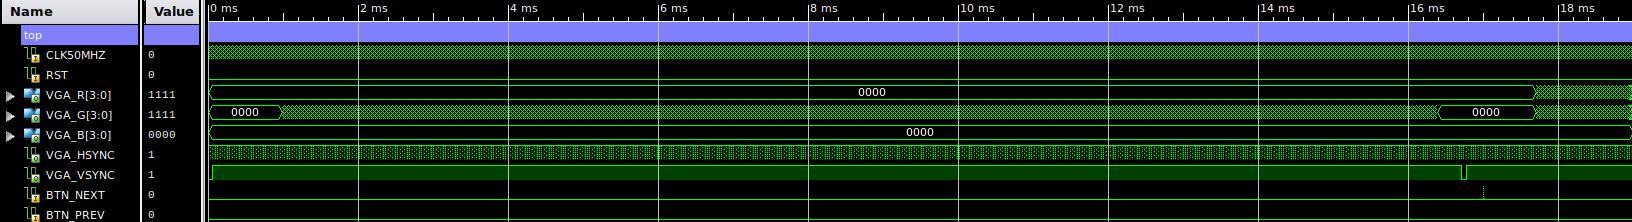
\includegraphics[width=15cm]{grafika/vga_sim.png}
   \caption{Przebieg symulacji}
\end{figure}

Zamieszczony jest fragment wyjścia logów dla domyślnych poziomów logowania.
\begin{lstlisting}[label=Vga_output,caption=Vga logs output]
  0 INFO3 [ TopTest.vga_behav_ ]  Oczekiwanie na poczatek nowej ramki.
  0 INFO3 [ TopTest.TopTestBench_.set_next.state ]  Stan sygnalow zostanie zmieniony. Obecny stan 'x' (0x x), spodziewany stan '0' (0x 0)
  0 INFO4 [ TopTest.TopTestBench_.set_next.state ]  Stan sygnalow zostal zmieniony. Obecny stan '0' (0x 0)
  0 INFO3 [ TopTest.TopTestBench_.set_prev.state ]  Stan sygnalow zostanie zmieniony. Obecny stan 'x' (0x x), spodziewany stan '0' (0x 0)
  0 INFO4 [ TopTest.TopTestBench_.set_prev.state ]  Stan sygnalow zostal zmieniony. Obecny stan '0' (0x 0)
Finished circuit initialization process.
500000 INFO3 [ TopTest.TopTestBench_ ]  Zadanie nastepnego koloru
500000 INFO3 [ TopTest.TopTestBench_.set_next.state ]  Stan sygnalow zostanie zmieniony. Obecny stan '0' (0x 0), spodziewany stan '1' (0x 1)
500000 INFO4 [ TopTest.TopTestBench_.set_next.state ]  Stan sygnalow zostal zmieniony. Obecny stan '1' (0x 1)
750000 INFO3 [ TopTest.TopTestBench_.set_next.state ]  Stan sygnalow zostanie zmieniony. Obecny stan '1' (0x 1), spodziewany stan '0' (0x 0)
750000 INFO4 [ TopTest.TopTestBench_.set_next.state ]  Stan sygnalow zostal zmieniony. Obecny stan '0' (0x 0)
64071000 INFO4 [ TopTest.vga_behav_ ]  Zsynchronizowano, rozpoczecie odbioru ramek.
96090000 INFO3 [ TopTest.vga_behav_.vga_behav_sync_ ]  Rozpoczecie odbioru nowego wiersza.
101850000 INFO4 [ TopTest.vga_behav_.vga_behav_sync_ ]  Nadawanie kolorow w wierszu
127470000 INFO5 [ TopTest.vga_behav_.vga_behav_sync_ ]  Nadano kolory w wierszu

128110000 INFO3 [ TopTest.vga_behav_.vga_behav_sync_ ]  Rozpoczecie odbioru nowego wiersza.
133870000 INFO4 [ TopTest.vga_behav_.vga_behav_sync_ ]  Nadawanie kolorow w wierszu
159490000 INFO5 [ TopTest.vga_behav_.vga_behav_sync_ ]  Nadano kolory w wierszu

160130000 INFO3 [ TopTest.vga_behav_.vga_behav_sync_ ]  Rozpoczecie odbioru nowego wiersza.
165890000 INFO4 [ TopTest.vga_behav_.vga_behav_sync_ ]  Nadawanie kolorow w wierszu
191510000 INFO5 [ TopTest.vga_behav_.vga_behav_sync_ ]  Nadano kolory w wierszu

...

16714470000 INFO3 [ TopTest.vga_behav_.vga_behav_sync_ ]  Rozpoczecie odbioru nowego wiersza.
16714470000 INFO3 [ TopTest.vga_behav_.vga_behav_sync_ ]  Rozpoczecie odbioru nowej ramki.
16720230000 INFO4 [ TopTest.vga_behav_.vga_behav_sync_ ]  Nadawanie wiersza
16745850000 INFO5 [ TopTest.vga_behav_.vga_behav_sync_ ]  Nadano  wiersz

...

17000750000 INFO3 [ TopTest.TopTestBench_ ]  Zadanie nastepnego koloru
17000750000 INFO3 [ TopTest.TopTestBench_.set_next.state ]  Stan sygnalow zostanie zmieniony. Obecny stan '0' (0x 0), spodziewany stan '1' (0x 1)
17000750000 INFO4 [ TopTest.TopTestBench_.set_next.state ]  Stan sygnalow zostal zmieniony. Obecny stan '1' (0x 1)
17001000000 INFO3 [ TopTest.TopTestBench_.set_next.state ]  Stan sygnalow zostanie zmieniony. Obecny stan '1' (0x 1), spodziewany stan '0' (0x 0)
17001000000 INFO4 [ TopTest.TopTestBench_.set_next.state ]  Stan sygnalow zostal zmieniony. Obecny stan '0' (0x 0)
17002010000 INFO5 [ TopTest.vga_behav_.vga_behav_sync_ ]  Nadano  wiersz

...

17675070000 INFO3 [ TopTest.vga_behav_.vga_behav_sync_ ]  Rozpoczecie odbioru nowego wiersza.
17680830000 INFO4 [ TopTest.vga_behav_.vga_behav_sync_ ]  Nadawanie wiersza
17706450000 INFO5 [ TopTest.vga_behav_.vga_behav_sync_ ]  Nadano  wiersz
17706510000 INFO4 [ TopTest.vga_behav_.vga_behav_sync_ ]  Nadawanie ramki
\end{lstlisting}



\section{Dodatki}

\subsection{Makefile}

Projekty można zsyntetyzować, przesymulować oraz przesłać na płytkę z wykorzystaniem programu GNU make. Skrypt wykorzystuje narzędzia Xilinxa dostępne z linii poleceń. W repozytorium podmodułu generic dostępny jest katalog 'makefile' z szablonami dla wszystkich projektów. Makefile'e projektów wyszczególniają swoje zależne pliki po czym załączają ogólny plik Makefile nazwany 'generic'.

\lstinputlisting[label=Makefile,caption=Makefile]{../projects/generic/makefile/generic}
\lstinputlisting[label=config.ut,caption=config.ut]{../projects/generic/makefile/config.ut}
\lstinputlisting[label=config.xst,caption=config.xst]{../projects/generic/makefile/config.xst}
\lstinputlisting{../projects/generic/makefile/impact_batch.tpl}

\subsubsection{DAC}
\lstinputlisting{../projects/dac/project/Makefile}

\subsubsection{Rotor}
\lstinputlisting{../projects/rotor/project/Makefile}

\subsubsection{Rs232}
\lstinputlisting{../projects/rs232/project/Makefile}

\subsubsection{VGA}
\lstinputlisting{../projects/vga/project/Makefile}


\linespread{1.3}
\selectfont

\end{document}
